\documentclass[preprint,11pt,a4paper,times]{elsarticle}
\usepackage{amsmath,amssymb,bm}
\usepackage{graphicx}
\usepackage{booktabs}
\usepackage{array}
\usepackage{tabularx}
\usepackage[font=small,labelfont=bf]{caption}
\usepackage{microtype}
\usepackage[hidelinks]{hyperref}
\graphicspath{{figs/}}
\setlength{\parskip}{2pt}

\renewcommand{\topfraction}{0.9}
\renewcommand{\bottomfraction}{0.8}
\renewcommand{\textfraction}{0.07}
\renewcommand{\floatpagefraction}{0.75}
\setcounter{topnumber}{3}
\setcounter{bottomnumber}{2}
\setcounter{totalnumber}{5}
\journal{International Journal of Heat and Mass Transfer}

\begin{document}

\begin{frontmatter}

\title{The Boussinesq--compressible gap in two-dimensional steady Rayleigh--B\'enard
convection is linear to leading order in the relative temperature contrast:\\
a factorised physics prior for surrogates}

\author[a]{Author(s)}
\address[a]{Affiliation(s)}

\begin{abstract}
Boussinesq-trained surrogates do not transfer across contrast. For
steady two-dimensional Rayleigh--B\'enard convection one parameter governs the difference, the
contrast $\varepsilon=\Delta T/T_0$. The Froude number is not free ($Fr^2=\varepsilon$), and a
24-fold change in $Ma$ moves the $O(Ma^2)$ correction by less than $10^{-5}$ in the retained
low-Mach equations. Over 627 paired solutions ($\varepsilon=0.02$--$1.9$), the relative
correction obeys $R=A\varepsilon^m$ with $m=1.023\pm0.018$, $0.995\pm0.019$, $1.024\pm0.077$ and
$1.009\pm0.015$ for $(u_x,u_y,\theta,p)$, a vanishing intercept and $\varepsilon^2$ curvature; the
$\theta$ amplitude is 0.010 wall-normalised, 0.034 zero-mean. It reproduces on another group's
public data ($\varepsilon\equiv1.2$), survives a second geometry and $Pr=4.38$, and
stays within 0.11 of unity in a twelve-sample 3-D check ($Ra=10^4$, $res=16$,
$\varepsilon\le1.2$). At $\varepsilon=1.2$ the integral Nusselt number changes by $0.6\%$, the local
wall flux by $4.25\%$. The prefactor is not universal: in $\theta$ it collapses on the peak
Boussinesq velocity across generators. Because $D=\varepsilon P(X)$, a surrogate predicts $P$ and multiplies: with $\varepsilon$ as input it improves $1.07$--$1.15\times$ over a FiLM-conditioned
network; without it, it still beats an $\varepsilon$-blind network by
$1.89\times$ and reuses single-$\varepsilon$ public data within a boundary family. One inference
takes 6.3\,ms; replacing the compressible member cuts a paired solve from 33.9\,s to
11.7\,s ($2.9\times$) and a 100-contrast sweep by 280.
\end{abstract}

\begin{keyword}
natural convection \sep Boussinesq approximation \sep low-Mach compressible flow \sep
physics-informed surrogate \sep neural operator \sep break symmetry
\end{keyword}

\end{frontmatter}

\section*{Nomenclature}
\vspace{-0.5em}
\begin{center}\small
\setlength{\tabcolsep}{4pt}
\resizebox{\textwidth}{!}{%
\begin{tabular}{@{}p{1.1cm}p{6.1cm}p{1.1cm}p{6.1cm}@{}}
\toprule
\multicolumn{2}{@{}l}{\emph{Roman}} & \multicolumn{2}{l}{\emph{Greek}}\\
\midrule
$A$ & prefactor of $R=A\varepsilon^{m}$ & $\beta$ & thermal expansion coefficient\\
$D$ & correction $Y-X$, the surrogate target & $\gamma$ & ratio of specific heats\\
$e$ & internal energy & $\Delta T$ & wall-to-wall temperature contrast\\
$Fr$ & Froude number, $Fr^{2}=\Delta T/T_{0}$ & $\varepsilon$ & relative contrast, $\Delta T/T_{0}$\\
$L$ & side length of the cavity & $\theta$ & normalised temperature\\
$m$ & scaling exponent & $\kappa$ & curvature, $R=A\varepsilon(1+\kappa\varepsilon)$\\
$Ma$ & Mach number & $\rho$ & density\\
$n$ & number of samples in a data set or split & $\bm\sigma$ & viscous stress tensor\\
$Nu$ & Nusselt number & & \\
$p$ & pressure & & \\
$P,\,Q$ & first- and second-order correction fields & & \\
$Pr$ & Prandtl number & & \\
$R$ & relative correction, $\|Y-X\|/\|Y\|$ & & \\
$Ra$ & Rayleigh number & & \\
$Re$ & Reynolds number, $(Ra/Pr)^{1/2}$ & & \\
$T$ & temperature, $T_{0}$ its reference value & & \\
$\bm u$ & velocity, $(u_x,u_y)$ & & \\
$\hat u$ & peak Boussinesq speed & & \\
$X,\,Y$ & Boussinesq and compressible solutions & $\mathcal{L}$ & linearised Boussinesq operator\\
\bottomrule
\end{tabular}}
\end{center}



\section{Introduction}
\label{sec:intro}

Steady natural convection is a workhorse of thermal engineering and it is expensive. A converged
pair of two-dimensional solves on a $64^2$ mesh costs 34\,s of wall clock on an eight-way desktop
(Sec.~\ref{sec:cost}); the three-dimensional problems that engineering actually needs cost hours to
days. That is the standard motivation for surrogate modelling, and the standard response is to
train a network that maps a cheap model's output to an expensive model's output
\citep{giacomini2026surrogates,meng2025physics}.

For convection the two models are not two arbitrary fidelities: they are the Boussinesq
(Oberbeck--Boussinesq) equations and the compressible low-Mach equations. Boussinesq is exact only
in the limit of vanishing relative temperature contrast; the corrections are $O(\beta\Delta T)$ and
have been characterised asymptotically for decades \citep{spiegel1960boussinesq,gray1976validity}.
Recent work makes the pair directly learnable. \citet{menglik2026neural} publish paired
Boussinesq$\to$compressible steady solutions in two dimensions (4000 training pairs plus held-out
splits, CC BY 4.0) and train a Fourier neural operator \citep{li2021fourier} to predict the
compressible field from the Boussinesq field. That data set---which we use as an independent
validation set in Secs.~\ref{sec:public}--\ref{sec:transfer}---contains exactly one
temperature contrast: $\Delta T=1.2$ at $T_0=1$.

The single-contrast design is the practical crux. A surrogate fitted on such a data set has learned
the correction at one operating point. At any other temperature contrast the Boussinesq input
already differs from the input seen in training, so the correction the network memorised is the
wrong correction---not merely an inaccurate one---and the only remedy on offer is to generate a
second paired data set, i.e.\ to pay again exactly the cost the surrogate was meant to remove. We
show in Sec.~\ref{sec:floor} that this is not a modelling failure that more capacity or a better
architecture can repair: it is an information barrier, and we measure it.

This paper makes the barrier explicit and then removes it.

\paragraph{What governs the gap} For the non-dimensionalisation used here the Froude number is not
free: $Fr^2=\beta\Delta T=\Delta T/T_0$ identically, and the Mach number enters the equations only
at $O(Ma^2)$ within the retained low-Mach equations (Sec.~\ref{sec:axis}, and measured: a
factor-24 change in $Ma$ moves the correction by less than $10^{-5}$). The break-symmetry group is therefore one-dimensional, and it has a
name: $\varepsilon=\Delta T/T_0$.

\paragraph{What the gap looks like} Expanding the compressible member in $\varepsilon$ gives an
$O(1)$ system that is term-by-term the Boussinesq system, plus an $O(\varepsilon)$ source produced
by the density-modulated inertia and by the non-solenoidal velocity field
$\nabla\cdot\bm{u}_1=\nabla\cdot(\theta_0\bm{u}_0)$. Because the linearised operator is
$\varepsilon$-independent, the correction factorises,
$Y-X=\varepsilon P(X)+\varepsilon^2Q(X)+\dots$, with a shape $P$ that does not rotate as
$\varepsilon$ moves (Sec.~\ref{sec:theory}). Measured over two decades of $\varepsilon$ (627
samples, Sec.~\ref{sec:law}) the relative correction obeys $R=A\varepsilon^m$ with $m=1.02$ in all
four channels (a window-averaged exponent: the same 627 points give $1.23$--$1.32$ when fitted from
$\varepsilon=0.8$ upwards, the $\varepsilon^2$ curvature of Sec.~\ref{sec:law}), a vanishing
intercept, and a prefactor whose weak Rayleigh-number trend reproduces in a second geometry and in
a third Prandtl number.

\paragraph{What it buys} Because the $\varepsilon$ dependence can be written outside the network, a
surrogate can predict $P(X)$ and multiply by $\varepsilon$ afterwards. Supplying $\varepsilon$ as
an input as well gives the largest gain---$1.07\times$ in extrapolation for the linear form and
$1.15\times$ for the quadratic form, relative to the strongest conditional baseline
(Sec.~\ref{sec:prior})---while removing it from the input costs a little accuracy but
is what lets a network trained on a public data set that exists at a single $\varepsilon$ be
applied, without retraining, to our $\varepsilon\in[0.2,1.9]$, where it reaches
$\mathrm{relL2}=0.093$ ($u_x$) against $0.144$ for the plain model at the same budget
(Sec.~\ref{sec:transfer}). The prior is also the cheaper model when data is scarce
(Sec.~\ref{sec:learning}: $1.4\times$ better than an $\varepsilon$-augmented baseline at $n=50$,
crossover near $n\approx300$), the network discovers the $\varepsilon^2$ curvature of the expansion
on its own (learned $\kappa=0.22$--$0.42$ in all four channels), and the same prior transfers
unchanged to a Fourier neural operator.

\subsection{Related work}
\label{sec:related}

\paragraph{Surrogates for convection} Reduced-order models replace the discretised equations by a
small number of modes; parametric dynamic mode decomposition is a representative recent example
\citep{huhn2022parametric}. Graph convolutional networks exploit the mesh and have been applied to
natural convection in annuli \citep{feng2024graph} and to geometry-adaptive steady convection with
physics-informed losses \citep{peng2023physics}. Operator learning removes the mesh-resolution
constraint: DeepONet approximates the solution operator from branch and trunk networks
\citep{lu2021learning}, physics-informed DeepONets add the residual to the loss
\citep{wang2021learning}, and Fourier neural operators (FNOs) learn a global convolution in Fourier
space \citep{li2021fourier}. FNOs have since been used for sparse-field reconstruction
\citep{zhao2023recfno}, real-time heat-pipe startup prediction \citep{yu2026fourier}, and
operator-level uncertainty quantification in cooling-channel optimisation \citep{sahin2023deep}.
Physics-informed neural networks \citep{raissi2019physics} and their heat-transfer variants
\citep{cai2021physics,jalili2023physics} take the opposite route: they solve one instance by minimising a PDE
residual, rather than learning a family of instances. Reviews of the numerical analysis and of the
application landscape are given by \citet{deryck2024numerical}, \citet{meng2025physics} and
\citet{luo2025physics}.

\paragraph{Physics priors and structure} A physics prior can enter as a residual penalty, as a
conservation law built into the architecture, or as an algebraic factorisation of the output. The
first two are well developed; the third is the subject of this paper. Residual-based corrector
operators add a learned correction on top of a neural-operator prediction and improve accuracy
without retraining the base operator \citep{jha2023residual,cao2023residual}. Physics-informed
extrapolation of deep operators has been demonstrated by adding sparse observations or residual
terms \citep{zhu2023reliable}, and transfer operator learning addresses distribution shift between
parameter regimes \citep{goswami2022deep}. Multi-fidelity surrogates combine cheap and expensive
data through LSTM corrections \citep{conti2022multi}, feature-adjacent physics-informed learning
\citep{chen2023feature} or transfer-learned FNOs \citep{lyu2023multi}. These methods reduce the
amount of high-fidelity data, but they still learn the parameter dependence from samples. The
present work differs in that the parameter dependence is derived, and only the spatial shape of the
correction is learned.

\paragraph{Boussinesq versus compressible convection} The Oberbeck--Boussinesq approximation and
its validity limits are classical \citep{spiegel1960boussinesq,gray1976validity}; the review of
\citet{ahlers2009heat} summarises the heat-transfer and large-scale dynamics of turbulent
Rayleigh--B\'enard convection. Non-Oberbeck--Boussinesq (NOB) effects have been measured under
strong temperature contrast \citep{yik2020turbulent}, in cryogenic helium \citep{macek2023assessing}
and in a water-filled differentially heated cavity \citep{pan2023non}. On the numerical side,
low-Mach compressible formulations for enclosed thermal convection have been developed and compared
with the Boussinesq limit \citep{zhang2023investigation,satake2024mathematical}, and the rigorous
derivation of the Oberbeck--Boussinesq approximation has recently been revisited
\citep{bella2023rigorous}. What is missing from this literature is a quantitative, closed-form
account of how the \emph{difference between the two solutions} scales with the temperature contrast,
and a surrogate design that uses that scaling. The works above either fix $\varepsilon$, treat it as
one more input channel, or study NOB corrections at the level of gross heat transfer; none turns the
correction into an output factorisation.

\paragraph{Contributions}
\begin{enumerate}
\item We identify the exact, one-dimensional break-symmetry parameter of the
Boussinesq--compressible pair and show the group is one-dimensional rather than two
(Sec.~\ref{sec:axis}).
\item We derive the correction's factorisation from an $\varepsilon$-expansion and verify all five
of its predictions numerically, including the divergence relation (Sec.~\ref{sec:theory}).
\item We calibrate the resulting law on 627 paired samples spanning two decades of $\varepsilon$, in
two geometries and two Prandtl numbers, and validate it on an independently generated public data
set---including the secondary Rayleigh-number trends (Secs.~\ref{sec:law}, \ref{sec:public},
\ref{sec:aspect}, \ref{sec:water}).
\item We measure what the gap does to the wall heat transfer: at $\varepsilon=1.2$ the integral
Nusselt number moves by $0.6\%$, while the local wall flux is redistributed by $4.25\%$
(Sec.~\ref{sec:nu}).
\item We turn the law into a surrogate design rule ($D=\varepsilon P(X)$), measure what it is worth
($1.07$--$1.15\times$ over the strongest conditional baseline), and show it makes an existing single-$\varepsilon$ public data set
reusable, with the end-to-end saving measured per pair ($2.9\times$) and for a 100-contrast
sweep ($2.8\times10^2$)
(Secs.~\ref{sec:baselines}--\ref{sec:transfer}, \ref{sec:cost}).
\end{enumerate}

All results are two-dimensional except the twelve-sample three-dimensional check of
Sec.~\ref{sec:3d}. Section~\ref{sec:limits} states the measured cost of the
three-dimensional problem on the same hardware and gives the concrete reasons we do not claim a 3-D
sweep.
\section{Problem, discretisation and the break-symmetry parameter}
\label{sec:problem}

\subsection{Two members per sample}
\label{sec:pair}

Every sample is a \emph{paired} steady solution of one physical configuration with two equation sets
on the same mesh ($res=64$, $L=1$, $Pr=0.71$, $\gamma=1.4$). The high-fidelity member $Y$ is the
compressible low-Mach formulation in $\bm w=(\bm u,T,\rho,p)$:
\begin{align}
\nabla\cdot(\rho\bm u)&=0,\label{eq:cmass}\\
\nabla\cdot(\rho\,\bm u\otimes\bm u)&=-\nabla p+\frac{1}{Re}\nabla\cdot\bm\sigma-\frac{1}{Fr^2}\rho\bm g,\label{eq:cmom}\\
\nabla\cdot(\rho E\bm u)&=\frac{\gamma}{Re\,Pr}\nabla^2e+\nabla\cdot(\bm P_{\mathrm{work}}\bm u)+O(Ma^2),\label{eq:cenergy}\\
\rho e&=\gamma Ma^2p+1,\qquad Re=(Ra/Pr)^{1/2}.\label{eq:ceos}
\end{align}
The low-fidelity member $X$ is the Boussinesq system in $(\bm u,T,p)$, written in the \emph{same}
free-fall scales:
\begin{align}
\nabla\cdot\bm u&=0,\label{eq:bmass}\\
\bm u\cdot\nabla\bm u&=-\nabla p+\left(\frac{Pr}{Ra}\right)^{1/2}\nabla^2\bm u+\theta\hat{\bm g},\label{eq:bmom}\\
\bm u\cdot\nabla T&=(Ra\,Pr)^{-1/2}\nabla^2T,\qquad \theta=\frac{T-T_0}{\Delta T}.\label{eq:benergy}
\end{align}
Both are solved with Taylor--Hood-type mixed elements, damped Newton iterations and a MUMPS
factorisation; steady states are reached by an adaptive march with a convergence guard. The
temperature boundary data are random Fourier wall temperatures with per-wall mode dials.

\subsection{$Fr$ is not a parameter, $Ma$ is negligible, $\varepsilon$ is the axis}
\label{sec:axis}

Table~\ref{tab:axis} lists the three candidates for a break-symmetry axis and what rules each one
out.

\begin{table}[htbp]
\centering
\small
\caption{The three candidate break-symmetry parameters. Only $\varepsilon$ survives as a free axis
in the present non-dimensionalisation. The $Ma$ row is a consistency check on the retained
equations, which drop the $O(Ma^2)$ term.}
\label{tab:axis}
\setlength{\tabcolsep}{3pt}
\begin{tabular}{@{}p{2.0cm}p{7.3cm}p{3.0cm}@{}}
\toprule
candidate & evidence & conclusion\\
\midrule
$Fr$ & the generators state $Fr^2=\beta\Delta T=\Delta T/T_0$ identically; the released 2-D code
pinned $Fr=1.095$, correct only at $\Delta T=1.2$ & not free; pinned-$Fr$ sweeps of $T_0/\Delta T$
are an artefact\\
$Ma$ & fixing $Ra$, $T_0$, $\Delta T$ and changing $Ma$ by $24\times$ leaves the correction
amplitude unchanged to five significant figures & $O(Ma^2)\approx10^{-6}$: unmeasurable\\
$\varepsilon=\Delta T/T_0$ & same boundary-condition seed stream, $\Delta T$ swept & the clean,
one-dimensional break-symmetry axis\\
\bottomrule
\end{tabular}
\end{table}


\subsection{The low-fidelity solution is exactly $\varepsilon$-blind}
\label{sec:blind}

$\theta$ and $Pr\,Ra$ are the only combinations that appear in the Boussinesq weak form; neither
$T_0$ nor $\Delta T$ appears alone. Hence, with the thermal data prescribed in $\theta$ and $Ra$
fixed, $X$ cannot depend on $\varepsilon$. This was verified to solver precision: across
20 configurations $\times$ 5 values of $\varepsilon$ (same $Ra$, bit-identical $\theta$ boundary
stream), the maximum relative deviation of $X$ is $9.77\times10^{-8}$.

\begin{quote}
\noindent\textbf{Corollary.} The correction $Y-X$ is information that is \emph{absent from the
surrogate's input}: no amount of capacity or training data can recover it from $X$ alone. The limit
is informational, not architectural (Sec.~\ref{sec:floor}).
\end{quote}

\section{Asymptotic theory: why the correction factorises as $\varepsilon P(X)$}
\label{sec:theory}

Write $T=T_0(1+\varepsilon\theta)$ with $\theta=O(1)$. With $\rho=1/T$ (the equation of state and
initial condition used here) and $Fr^2=\varepsilon$, the buoyancy source is
\begin{equation}
\frac{\rho\bm g}{\varepsilon}=\frac{\bm g}{\varepsilon}-\theta\bm g+\varepsilon\theta^2\bm g+\dots,
\label{eq:buoyancy}
\end{equation}
so the $O(1)$ balances are
\begin{align}
\nabla\cdot\bm u_0&=0,\label{eq:o1mass}\\
\bm u_0\cdot\nabla\bm u_0&=-\nabla\tilde p_0+Re^{-1}\nabla^2\bm u_0+\theta_0\hat{\bm g},\label{eq:o1mom}\\
\bm u_0\cdot\nabla\theta_0&=(Re\,Pr)^{-1}\nabla^2\theta_0,\label{eq:o1energy}
\end{align}
which is term-by-term the Boussinesq system solved as $X$ ($Re^{-1}=(Pr/Ra)^{1/2}$). The
correction at $O(\varepsilon)$ is driven by the density modulation:
\begin{align}
\nabla\cdot\bm u_1&=\nabla\cdot(\theta_0\bm u_0),\label{eq:div1}\\
\nabla\cdot(\bm u_1\otimes\bm u_0+\bm u_0\otimes\bm u_1-\theta_0\bm u_0\otimes\bm u_0)
&=-\nabla\tilde p_1+Re^{-1}\nabla^2\bm u_1+\theta_1\hat{\bm g}+\theta_0^2\hat{\bm g}.\label{eq:mom1}
\end{align}
Since $\mathcal{L}$, the linearisation of the Boussinesq operator about $X$, does not contain $\varepsilon$,
\begin{equation}
D=Y-X=-\varepsilon \mathcal{L}^{-1}S_1[X]-\varepsilon^2\mathcal{L}^{-1}S_2[X]+\dots
=\varepsilon P(X)+\varepsilon^2Q(X)+\dots
\label{eq:factor}
\end{equation}
Five predictions follow, and all five hold; Table~S1 of the supplementary material lists them and
their measured values.



The drift of the divergence check with $\varepsilon$ ($0.994\to0.901$) is the truncated
$\varepsilon^2$ term, which is exactly what the fifth row of Table~S1 measures independently.

\paragraph{Domain of validity} $\varepsilon<2$, since the cold wall $T_c=T_0-\Delta T/2$ must be
positive.
\section{Data sets and protocols}
\label{sec:data}

Table~\ref{tab:data} lists the data sets.

\begin{table}[htbp]
\centering
\footnotesize
\setlength{\tabcolsep}{4pt}
\caption{Data sets used in this study. The public sets are from
\citet{menglik2026neural}.}
\label{tab:data}
\begin{tabular}{@{}p{3.0cm}c p{4.0cm}p{2.8cm}@{}}
\toprule
set & $n$ & what varies & purpose\\
\midrule
random-BC & 600 & $Ra\sim\log U[10^2,10^6]$, $\varepsilon\sim U[0.2,1.9]$, 134 wall-mode
families & calibrate the law, train surrogates\\
$\varepsilon\to0$ checks & 27 & $\varepsilon=0.02/0.05/0.10$ $\times$ $Ra=10^3/10^4/10^5$ &
test $R(0)=0$\\
paired & $20\times5$ & only $\varepsilon$; $Ra$ and the $\theta$ boundary stream fixed within a
configuration & exact $\varepsilon$-blind floor, shape invariance\\
aspect 2:1 & 104 & same law, geometry $2\times1$ & external validity\\
tight rerun & 10 & the 10 worst-converged samples, tolerance $10^{-6}\to10^{-8}$ & noise control\\
public, random walls \citep{menglik2026neural} & $4000+2\times200$ & $\varepsilon\equiv1.2$; the
two held-out splits differ in the range of the wall dials & external
validation, cross-data-set transfer\\
public, classical cavity \citep{menglik2026neural} & $5000+200$ & constant hot/cold side walls,
adiabatic top and bottom, $\varepsilon\equiv1.2$ & external validation of the prefactor\\
$Pr=4.38$ (this work) & 104 & $Pr=4.38$; BC/$Ra$/$\varepsilon$ draws bit-identical to 104 of the
random-BC samples & test of the fluid axis\\
\bottomrule
\end{tabular}
\end{table}

Surrogates use residual learning $\hat Y=X+\mathcal{N}(\cdot)$, a U-Net of width 32 (or an FNO2d
with 12 modes, width 32, four layers, 1.19\,M parameters), Adam with cosine annealing, 200 epochs,
batch 16, and targets normalised per channel. Inputs and targets are scaled per channel by
standard deviations of the training split; in the cross-data-set transfer experiment the target
pool is scaled by the standard deviation of its own inputs, which uses no labels. Two splits are used throughout:
extrapolation (train $\varepsilon\le1.3$, test $\varepsilon>1.3$, $n=218$) and
interpolation (stratified 2:1 in $\varepsilon$, $n=200$). Errors are the per-channel
relative $L_2$ error against $Y$; ``floor'' means $\hat Y=X$.

Tables that support the argument but are not needed in its flow---the asymptotic predictions, the
two-parameter fits, the exact single-$\varepsilon$ transfer matrix, the learning curve, the public
data splits, the prefactor--velocity law and the map from scripts to reported numbers---are
collected in the supplementary material; they are cited where they are used.

\paragraph{Temperature normalisation} Eq.~\eqref{eq:benergy} defines the zero-mean variable
$\theta=(T-T_0)/\Delta T$. The public release and our own pipeline store $T/T_0$ and evaluate every
temperature error on the wall-normalised $\theta_w=(T-T_c)/\Delta T\in[0,1]$, which differs from
$\theta$ by the constant $1/2$. All $R_\theta$, $A_\theta$ and $p_\theta$ quoted below are in the
wall-normalised convention. The same field difference reads $0.0220$ wall-normalised against
$0.0869$ zero-mean on the public random-wall test split, and $0.0836$ against $0.1628$ on the
classical cavity; the two conventions must not be mixed. In Table~\ref{tab:law} the $\theta$
amplitude is therefore listed in both, $0.010$ wall-normalised and $0.034$ zero-mean.

\section{Results}
\label{sec:results}

\subsection{The $\varepsilon$-law, calibrated over two decades}
\label{sec:law}

Fig.~\ref{fig:law} shows the collapse and Table~\ref{tab:law} collects the fits.

\begin{table}[htbp]
\centering
\small
\caption{Power-law fit $R=A\varepsilon^m$ over the full two-decade window (627 samples). The
intercept is fitted separately on the small-$\varepsilon$ subset ($\varepsilon\le0.5$). For $\theta$
the amplitude is given in both conventions, wall-normalised/zero-mean.}
\label{tab:law}
\begin{tabular}{@{}lcccc@{}}
\toprule
channel & $R=A\varepsilon^m$ & $A$ & $R^2$ & intercept ($\varepsilon\le0.5$)\\
\midrule
$u_x$ & $m=1.023\pm0.018$ & 0.147 & 0.84 & $+0.0003\pm0.0047$\\
$u_y$ & $m=0.995\pm0.019$ & 0.193 & 0.82 & $+0.0030\pm0.0062$\\
$\theta$ & $m=1.024\pm0.077$ & 0.010/0.034 & 0.22 & $-0.0003\pm0.0012$\\
$p$ & $m=1.009\pm0.015$ & 0.148 & 0.87 & $+0.0016\pm0.0030$\\
\bottomrule
\end{tabular}
\end{table}

\begin{figure}[htbp]
\centering
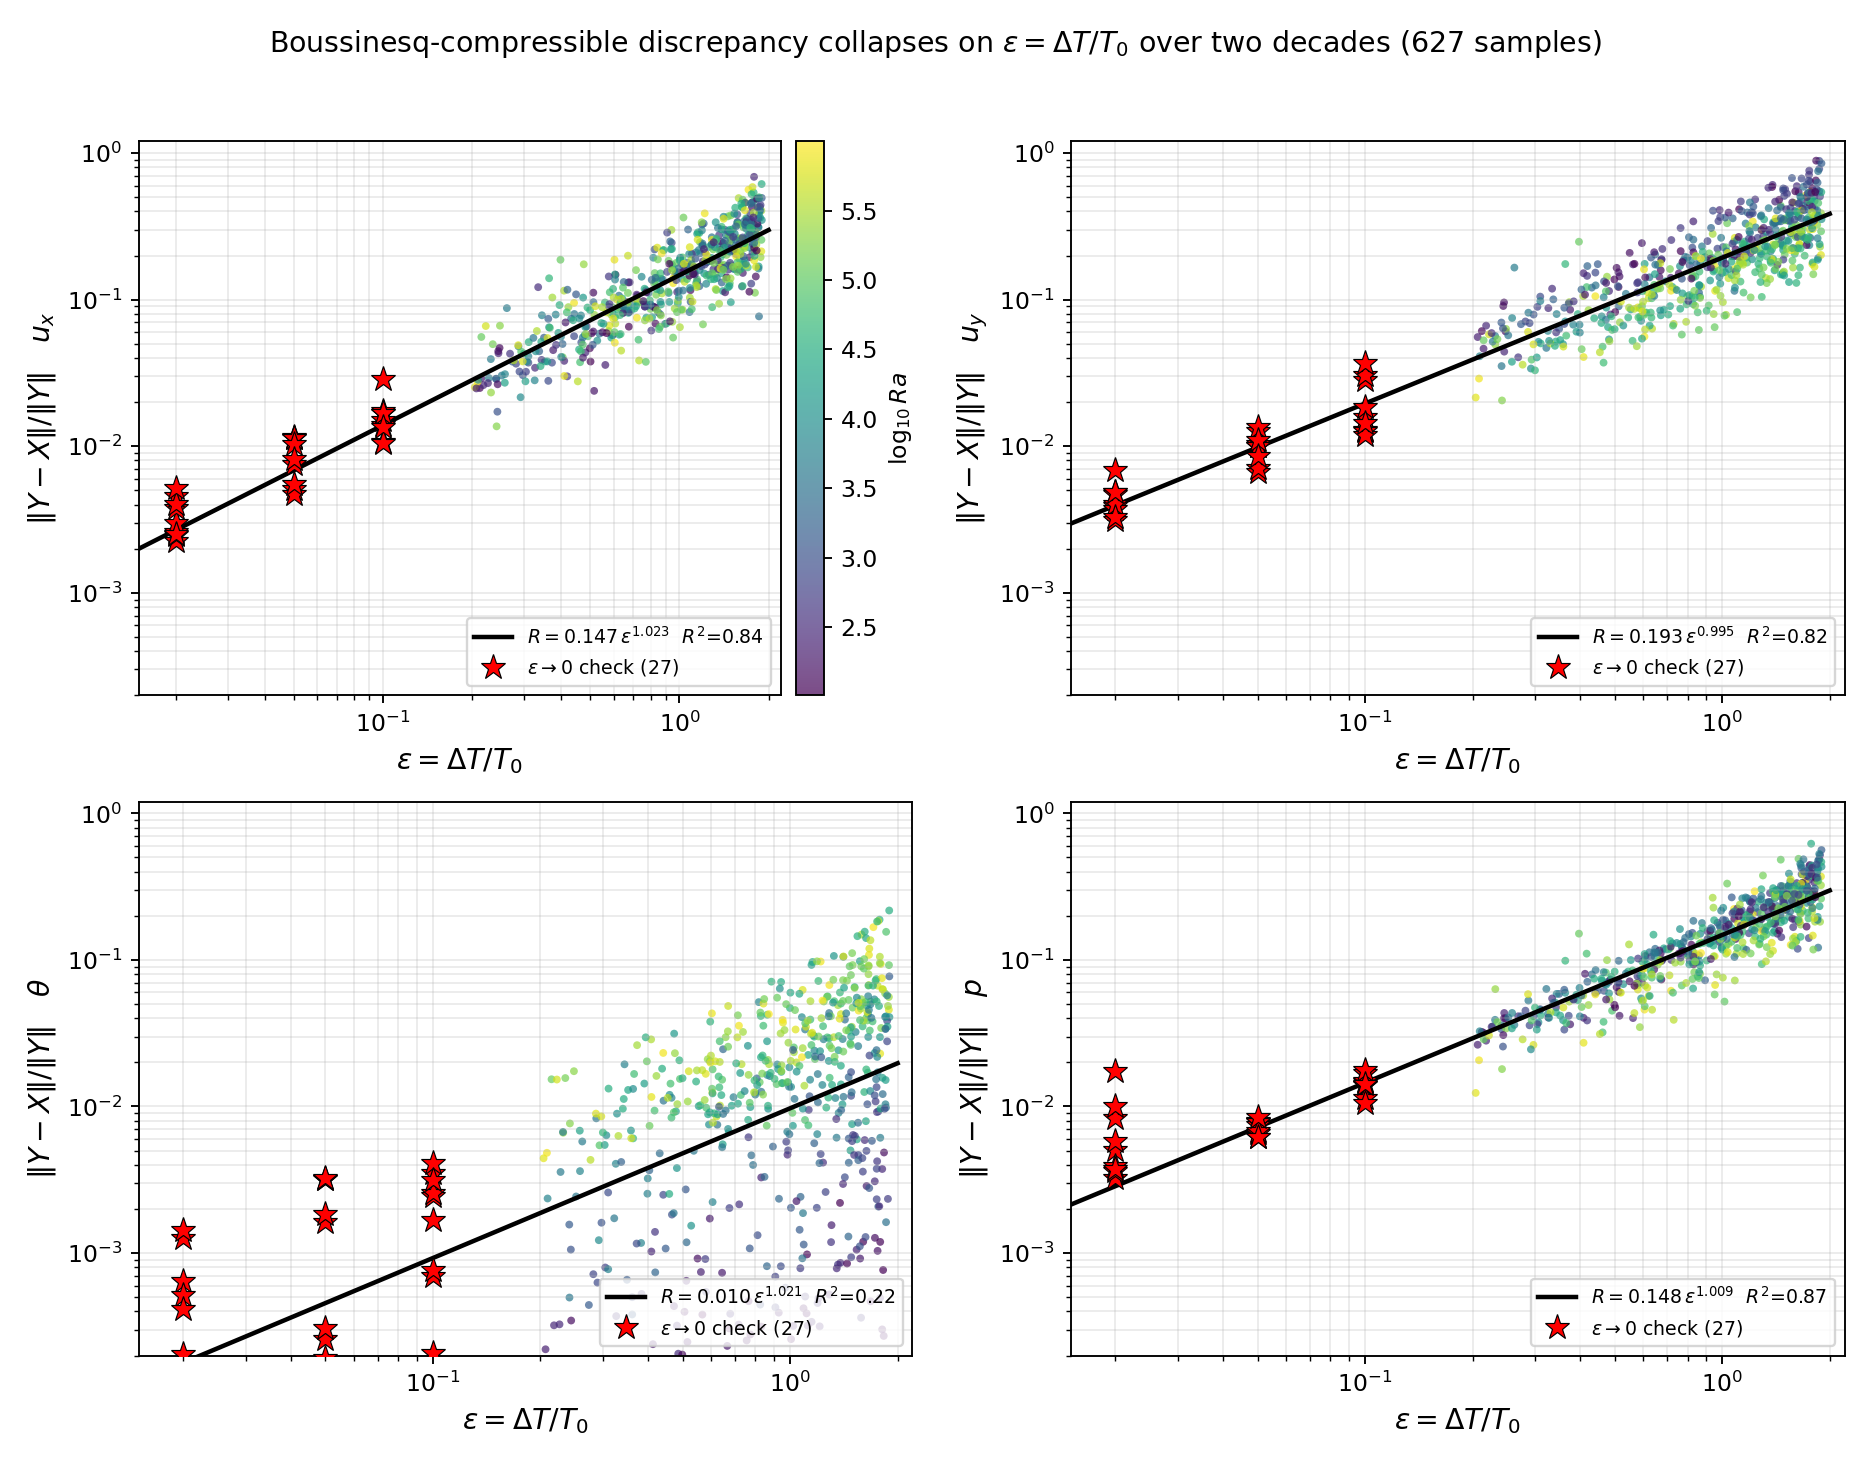
\includegraphics[width=0.95\textwidth]{fig1_law.png}
\caption{The Boussinesq--compressible discrepancy collapses on
$\varepsilon=\Delta T/T_0$ over two decades. Points: 600 random-boundary-condition samples,
coloured by $\log_{10}Ra$; stars: the 27 independent small-$\varepsilon$ checks. Lines: the
power-law fits of Table~\ref{tab:law}.}
\label{fig:law}
\end{figure}

\paragraph{The exponent is window-averaged, and the curvature is real} The fit above uses the full
two decades, including the 27 check points at $\varepsilon\le0.1$ where $R$ is closest to its
linear limit. Fitting only $\varepsilon\ge0.8$ gives
$m=1.23\pm0.08/1.25\pm0.08/1.21\pm0.34/1.32\pm0.06$, and fitting each of the 20 paired
configurations separately over $\varepsilon\in[0.4,1.9]$ gives a median
$m=1.31/1.17/1.21/1.45$ (median $R^2=0.98$, \path{code/audit_v2.py}). That is the signature of
$R=A\varepsilon(1+\kappa\varepsilon)$ rather than of an exact power: a power law fitted to a curved
function over a window that excludes small $\varepsilon$ returns $m\approx1+\kappa\langle
\varepsilon\rangle$. The quadratic fit $R=a\varepsilon+c\varepsilon^2+b$ gives $c>0$ in all four
channels ($u_x$: $+0.0513\pm0.0133$, $3.9\sigma$; $u_y$: $+0.0695$; $\theta$: $+0.0060$; $p$:
$+0.0539$) with $\kappa=c/a=0.70/0.83/0.42/0.73$. We therefore state the law as first order
in $\varepsilon$, $R=A\varepsilon(1+O(\varepsilon))$, quote $m=1.02$ as the number a wide-window
fit returns, and note that the network recovers the $\varepsilon^2$ curvature with the same sign and order of magnitude
(Sec.~\ref{sec:prior}, $\kappa=0.22$--$0.42$) and by the mode expansion (Sec.~\ref{sec:theory},
$\varepsilon^1+\varepsilon^2$ carry 99.0\% of the correction energy).



\begin{itemize}
\item $\varepsilon$-scaling is geometry-independent; the prefactor $A$ is not ($0.147\to0.175$ for
$u_x$, $0.148\to0.222$ for $p$, $0.193\to0.175$ for $u_y$, $0.010\to0.008$ for $\theta$).
\item Boundary-condition families barely matter \emph{inside this family}: 134 wall-mode families,
133 free dummies. Adding them to the $\varepsilon$-only fit raises the adjusted $R^2$ by 2.3 pp
($p$), 2.9 pp ($u_y$), 3.3 pp ($u_x$) and 8.5 pp ($\theta$)---the $\varepsilon$-scaling is not an
artefact of which wall modes were drawn (\path{code/audit_numbers.py}).
\item The $\theta$ channel needs one extra, cheaply available parameter, the advection strength of
the base flow $\chi=\|\bm u\|\|\nabla\theta\|/\|\theta\|$:
$R_\theta=\varepsilon(-0.0037+0.226\chi)$, $R^2$ $0.185\to0.778$ (Spearman 0.902), i.e.\
$R_\theta\approx0.23\varepsilon\chi$. For $u_x/u_y/p$ adding $\chi$ does nothing. A single-input
form of the same statement, $R_\theta/\varepsilon=c\hat u^a$, is calibrated on two independent
generators in Sec.~\ref{sec:public} and carries the same information with $R^2=0.90$.
\item A pressure-channel preprocessing bug had to be fixed first (Sec.~\ref{sec:pressure}).
\end{itemize}
\subsection{A pressure-channel artefact, and why it mattered}
\label{sec:pressure}

Pairing the two members' \emph{raw} pressures mixes units: the compressible raw pressure carries a
hydrostatic ramp $12\times$ larger than its dynamic part, and the two weak forms use opposite
pressure sign conventions. Before the fix the per-sample median of $|X_p|/|Y_p|$ was $0.065$ and
that of $\cos(X_p,Y_p)$ was $-0.105$, and the $p$-channel ``law'' was a constant
($R_p\approx1.0$). Applying the recipe used by the public data set---subtract the mean, remove a
least-squares linear-in-$y$ fit, flip the sign of the Boussinesq member---gives $0.960$ and
$\cos=+0.991$ under the same median convention, against $0.929$ and $+0.986$ for the public
training set, i.e.\ we now match their pairing to within 3\% (\path{code/audit_v2.py}). The
channel then obeys the same law as the velocities ($A=0.148$, $m=1.009$). All $p$-channel numbers
reported here are post-fix.

\subsection{The $\varepsilon$-blind ceiling, measured exactly}
\label{sec:floor}

Within a configuration $X$ is identical for all $\varepsilon$, so an $\varepsilon$-blind model must
emit one field $F$ for every $\varepsilon$ it is applied at (Fig.~\ref{fig:floor},
Table~\ref{tab:floor}). Two reference protocols are exact
rather than fitted: (A) train at the one $\varepsilon$ a published data set offers (here
$\varepsilon=1.2$) and apply it everywhere, error $\|Y(\varepsilon)-Y(1.2)\|/\|Y(\varepsilon)\|$;
(B) the single field that best serves the whole range, the $\varepsilon$-mean of $Y$. (B) is a
least-squares compromise over the $\varepsilon$-range, not a per-$\varepsilon$ lower
bound---a field tuned to $\varepsilon=0.8$ gives $0.067$ at $\varepsilon=0.4$, better than (B)'s
$0.170$ there, and below $\varepsilon\approx0.8$ doing nothing beats both. Median over 20
configurations, channels $u_x/u_y/\theta/p$:

\begin{table}[htbp]
\centering
\footnotesize
\setlength{\tabcolsep}{4pt}
\caption{The exact $\varepsilon$-blind floor. Protocol (A) is what a single-$\varepsilon$ public
data set forces; protocol (B) is the best single field over the whole range. Entries are medians
over 20 configurations, ordered $u_x/u_y/\theta/p$.}
\label{tab:floor}
\setlength{\tabcolsep}{3pt}
\begin{tabular}{@{}c p{3.7cm}p{3.7cm}p{3.7cm}@{}}
\toprule
$\varepsilon$ & do nothing ($\hat Y=X$) & (A) train at $\varepsilon=1.2$ only & (B)
$\varepsilon$-mean field\\
\midrule
0.4 & 0.060/0.098/0.009/0.061 & 0.143/0.219/0.021/0.146 & 0.170/0.244/0.023/0.177\\
0.8 & 0.127/0.203/0.019/0.129 & 0.078/0.118/0.011/0.082 & 0.108/0.143/0.013/0.126\\
1.2 & 0.211/0.328/0.030/0.220 & 0/0/0/0 & 0.035/0.036/0.003/0.051\\
1.6 & 0.322/0.481/0.044/0.347 & 0.112/0.151/0.014/0.131 & 0.079/0.123/0.012/0.085\\
1.9 & 0.472/0.616/0.058/0.547 & 0.251/0.304/0.031/0.346 & 0.225/0.286/0.028/0.281\\
\bottomrule
\end{tabular}
\end{table}

\begin{figure}[htbp]
\centering
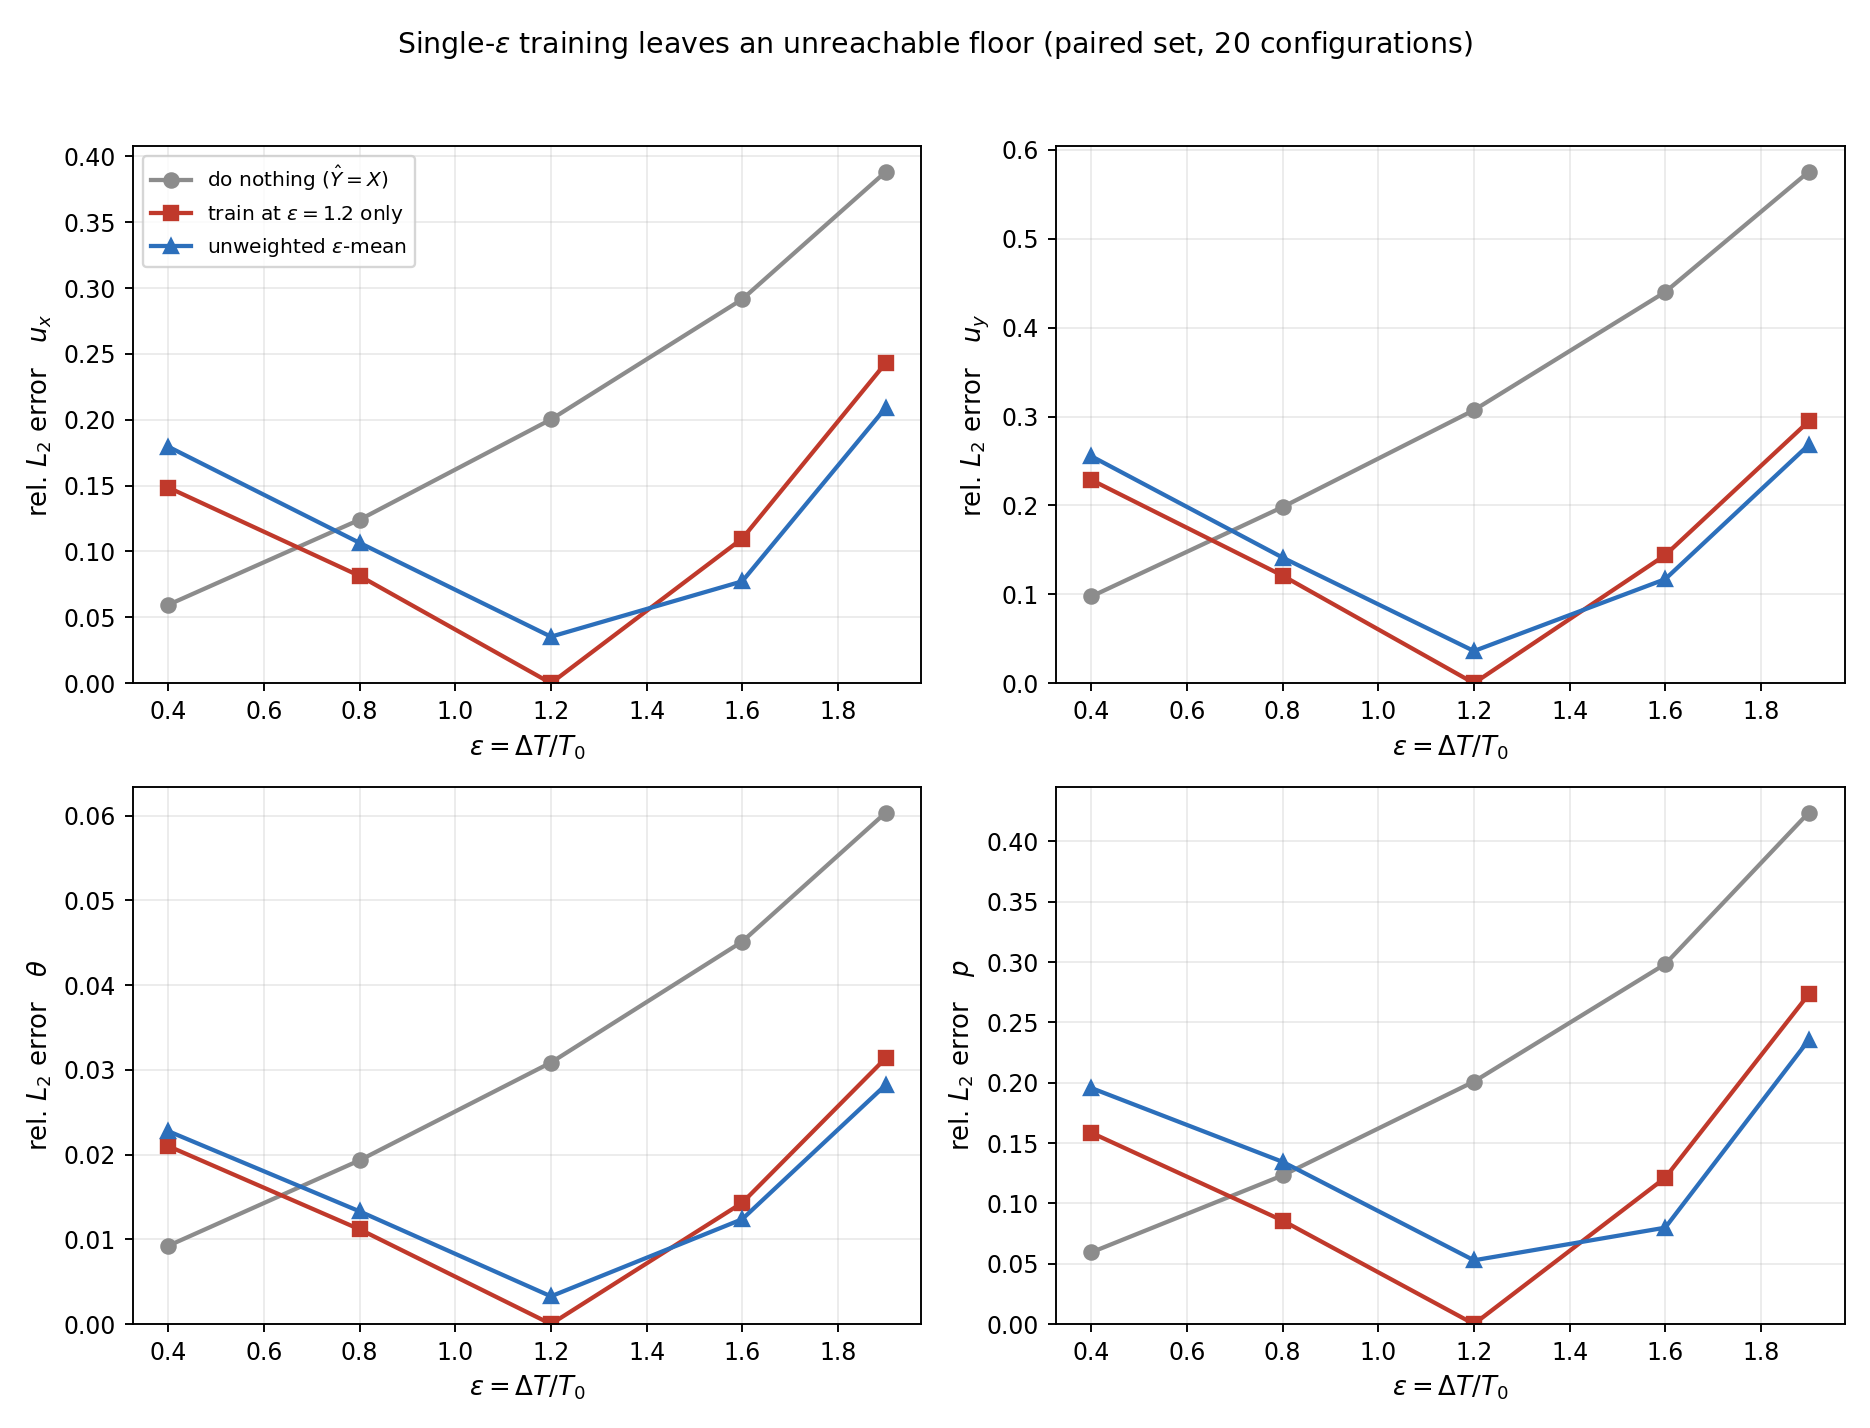
\includegraphics[width=0.95\textwidth]{fig2_floor.png}
\caption{Single-$\varepsilon$ training leaves an unreachable floor. Curves show ``do nothing'',
training at $\varepsilon=1.2$ only, and the best $\varepsilon$-blind field, for the 20 paired
configurations.}
\label{fig:floor}
\end{figure}

Protocol (A) is what a single-$\varepsilon$ public data set forces: 25\% ($u_x$), 30\% ($u_y$) and
35\% ($p$) error at $\varepsilon=1.9$, 8\% ($u_x$) already at $\varepsilon=0.8$, and---the point
for practice---at $\varepsilon=0.4$ ``do nothing'' is \emph{better} than it, and the two cross
between $\varepsilon=0.4$ and $0.8$. Protocol (B), the least-squares compromise over the range and
therefore the best a single $\varepsilon$-blind field can do on average, still leaves
$22.5/28.6/28.1\%$ at $\varepsilon=1.9$. The whole effect is one line of arithmetic, and the paired
set measures it exactly (\path{code/exp_paired_final.py}; the diagonal is identically zero
because the same $\varepsilon$ is the same solution): the full $5\times5$ matrix is Table~S3 of
the supplementary material.



The error is set by the distance in $\varepsilon$ and by nothing else---which is precisely the
quantity $\varepsilon P(X)$ puts back into the model.

\subsection{Network baselines: the correction is information, not capacity}
\label{sec:baselines}

\begin{table}[htbp]
\centering
\footnotesize
\setlength{\tabcolsep}{3pt}
\caption{Surrogate ablation on the two fixed splits (U-Net, width 32, 200 epochs, mean of three
seeds; largest standard deviation over all cells 0.0051). A sees only the four Boussinesq fields;
B also receives $\varepsilon$ as a constant input channel; P1 multiplies $\varepsilon$ outside the
network but still reads it as an input; P2 adds a learned quadratic factor; P3 removes
$\varepsilon$ from the input entirely. Errors are per-channel relative $L_2$ errors against $Y$.
The curvature learned by P2 (seed 0) is $\kappa=0.418/0.314/0.334/0.314$ (extrapolation) and
$0.295/0.224/0.255/0.219$ (interpolation), for $u_x/u_y/\theta/p$; the three-seed means are
$0.418/0.321/0.343/0.338$ and $0.286/0.232/0.252/0.265$. The own-data row of
Table~\ref{tab:transfer} is the P3 architecture trained with 150 epochs and one seed, the protocol
of the public-transfer rows; this table uses 200 epochs and three seeds; the same architecture therefore differs between the
tables by 2--6\% in extrapolation and 6--12\% in interpolation.}
\label{tab:ablation}
\begin{tabular}{@{}p{3.2cm}p{1.0cm}ccccc@{}}
\toprule
split & channel & A & B & P1 & P2 & P3\\
\midrule
extrapolation ($n=218$) & $u_x$ & 0.2289 & 0.1508 & 0.0937 & 0.0867 & 0.1214\\
 & $u_y$ & 0.2733 & 0.1725 & 0.1060 & 0.0951 & 0.1277\\
 & $\theta$ & 0.0406 & 0.0255 & 0.0141 & 0.0131 & 0.0161\\
 & $p$ & 0.2689 & 0.1791 & 0.1126 & 0.1007 & 0.1682\\
interpolation ($n=200$) & $u_x$ & 0.1530 & 0.0673 & 0.0545 & 0.0507 & 0.0732\\
 & $u_y$ & 0.1796 & 0.0714 & 0.0524 & 0.0488 & 0.0749\\
 & $\theta$ & 0.0261 & 0.0097 & 0.0078 & 0.0073 & 0.0092\\
 & $p$ & 0.1792 & 0.0667 & 0.0454 & 0.0410 & 0.0893\\
\bottomrule
\end{tabular}
\end{table}

Table~\ref{tab:ablation} reports a U-Net of width 32, 200 epochs, mean of three seeds, identical
protocol for all columns (largest standard deviation over every cell: 0.0051).



Model A's error on the extrapolation split (0.2289) is within 2\% of the $\varepsilon$-mean field
of the paired set at $\varepsilon=1.9$ (0.2249, Sec.~\ref{sec:floor}), although the two are measured
on different data sets; the agreement is consistent with a ceiling that is informational rather
than architectural. Shallow learners plateau in
the same place. A linear ridge regression and an RBF kernel ridge on the raw four-field
input---the same information the network gets---reach $u_x$ 0.2282 and 0.2222 in extrapolation, and
adding $\varepsilon$ as an extra column barely moves them (0.2188 and 0.2171, against 0.0937 for
the structured model), because neither can represent a product of an $\varepsilon$-scale with a
spatial field. A classical POD-ROM (44--52 modes, 99.9\% of the snapshot energy) whose coefficients
are regressed on $(\log_{10}Ra,\varepsilon)$ lands at 0.2937 with $\varepsilon$ and 0.3001 without,
i.e.\ at the level of doing nothing, and a purely linear surrogate that also sees the POD
coefficients of $X$ reaches only 0.2318. The plateau is not capacity---it is that the quantity to be
added is absent from the input (\path{code/exp_shallow.py}, \path{code/exp_pod.py}).
\paragraph{A first-order perturbation baseline} If the correction is linear in $\varepsilon$, the
obvious alternative is to solve the linearised equations once and scale. We evaluated that
baseline on the 20 configurations of the $\varepsilon$ scan: $P=(Y-X)/\varepsilon$ at $\varepsilon=0.4$, the smallest
contrast available there, which is a finite-difference evaluation of $-\mathcal{L}^{-1}S_1[X]$ with
an $O(0.4)$ error in $P$, and predicted $\hat Y=X+\varepsilon P$. The error is
$5.3/5.5/0.5/5.7\%$ at $\varepsilon=1.2$ and $22/26/2.9/26\%$ at $\varepsilon=1.9$, against a
do-nothing floor of $42/60/7.3/41\%$; the linear response removes about half the gap at the largest
contrast and leaves the other half to the $O(\varepsilon^2)$ term. Obtaining $P$ costs one
compressible solve (median 30\,s on these configurations), against 6.3\,ms for the network, and the
network learns the curvature that the linear solve cannot produce (Table~\ref{tab:ablation}).

\subsection{The physics prior: $D=\varepsilon P(X)$}
\label{sec:prior}

Same backbone, only the output structure changes (Table~\ref{tab:ablation} of
Sec.~\ref{sec:baselines}; $\varepsilon$ still read from a constant channel, target still $D$).



\begin{figure}[htbp]
\centering
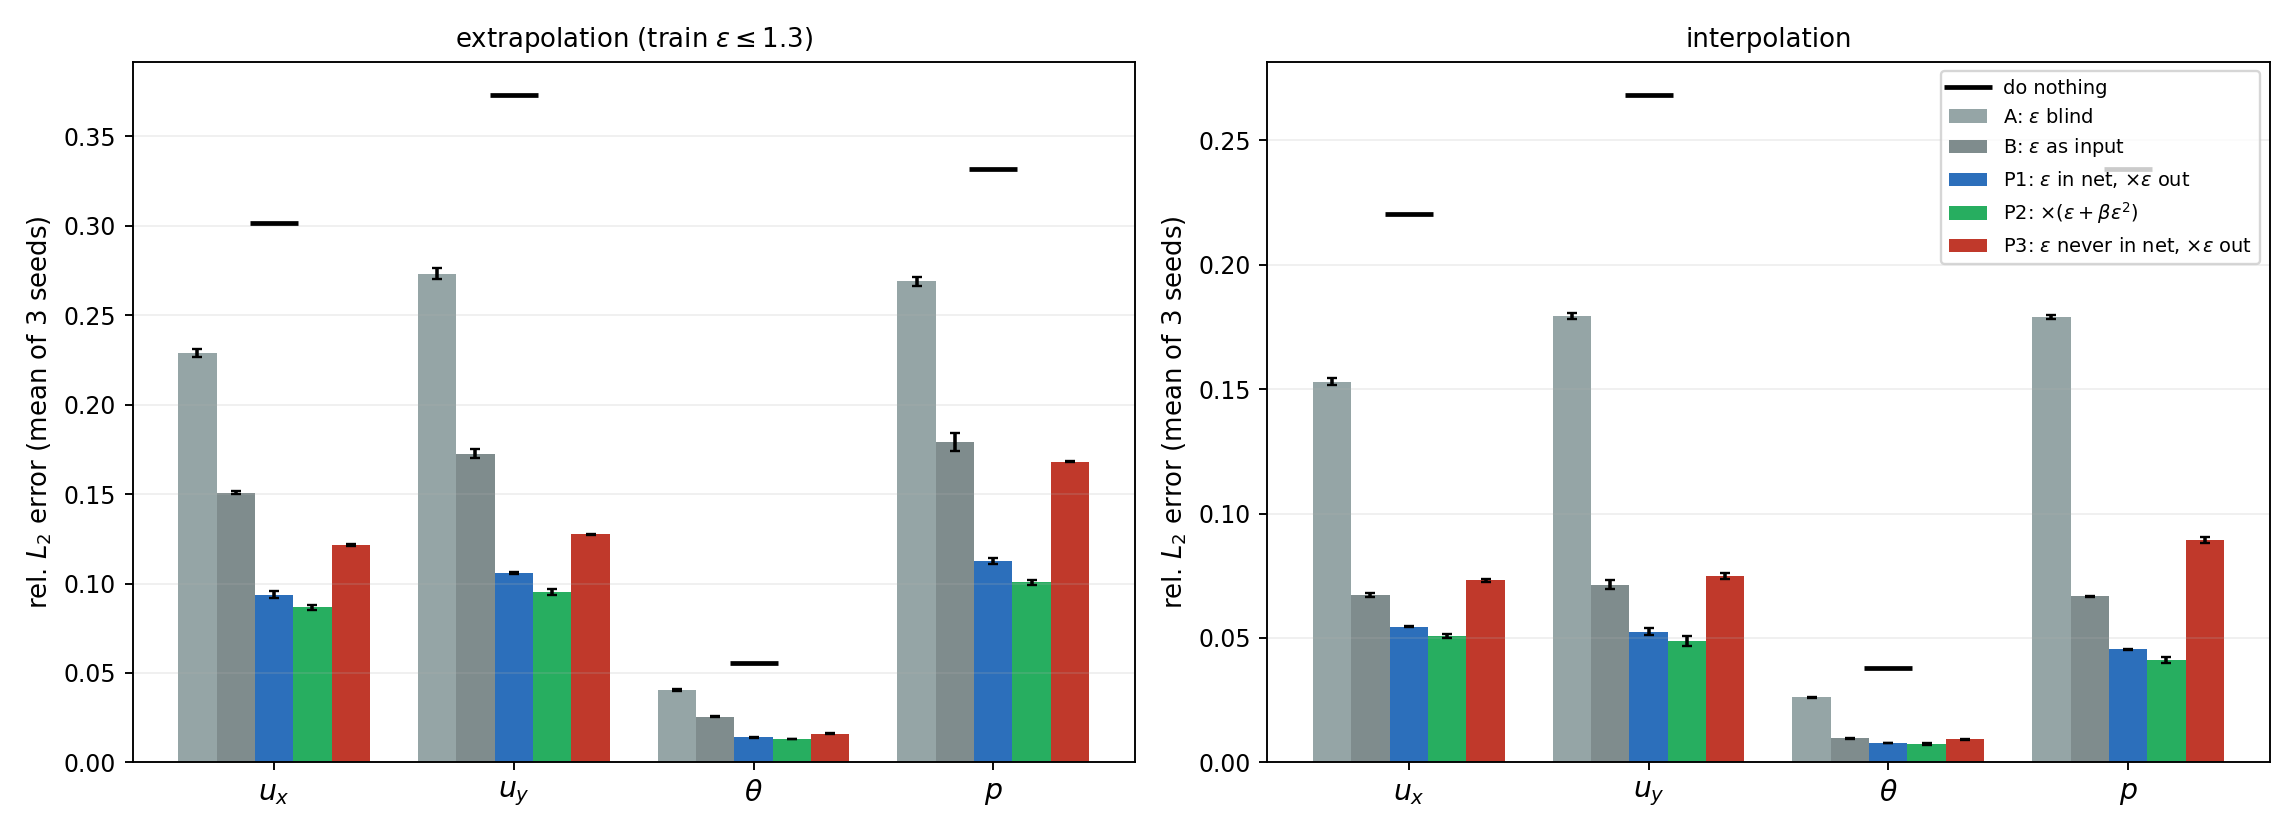
\includegraphics[width=0.98\textwidth]{fig3_prior.png}
\caption{The prior ablation for extrapolation (left) and interpolation (right). A: $\varepsilon$-blind.
B: $\varepsilon$ as input. P1: $\varepsilon$ in the network, multiplied outside. P2: learned
$(\varepsilon+\kappa\varepsilon^2)$ factor. P3: $\varepsilon$ never enters the network.}
\label{fig:prior}
\end{figure}

Three things happen at once (Table~\ref{tab:ablation}, Fig.~\ref{fig:prior}). In extrapolation the
factorised output beats a plain network that reads $\varepsilon$ from a constant input channel by
$1.61\times$ ($u_x$) and $1.59$--$1.81\times$ in the other channels, and the quadratic form adds a
further 7.1--10.6\% on top. That channel is a weak way to condition a network. A FiLM-conditioned
U-Net, which modulates every block with $\varepsilon$, reaches $0.1001\slash0.1155\slash0.0164\slash0.1251$ in
extrapolation and $0.0544\slash0.0496\slash0.0073\slash0.0428$ in interpolation, so against that baseline the
factorised output gains $1.07\times$ and the quadratic form $1.15\times$ in $u_x$. Removing $\varepsilon$ from the input as well costs accuracy relative to P1 and FiLM---0.1214
against 0.0937 and 0.1001 in $u_x$---but still beats the $\varepsilon$-blind network
($1.89\times$); what it buys is the property P1 cannot have, a network that can be trained at
one $\varepsilon$ and applied at another (Sec.~\ref{sec:transfer}). Finally, the network
\emph{discovers} a positive curvature on its own, $\kappa=0.22$--$0.42$, the same sign and order as
the $\varepsilon^2$ term of the expansion in Sec.~\ref{sec:theory}---an independent check of the
asymptotic expansion.

\paragraph{Practical form} The prior costs two lines of code: train any regressor $\mathcal{N}$ on the
ratio $D/\varepsilon$ instead of on $D$, and at run time return $\hat Y=X+\varepsilon\,\mathcal{N}(X)$
after evaluating the Boussinesq member (or a surrogate for it) to obtain $X$. Supplying
$\varepsilon$ to $\mathcal{N}$ as well is the most accurate form (P1, $1.07\times$ over a FiLM-conditioned
network); leaving it out (P3) costs accuracy at fixed data but is what lets one network serve
every contrast for which the prefactor is unchanged, because $\mathcal{N}$ then sees only $X$ and
re-learns the prefactor from the flow rather than from a tabulated value.

A Fourier neural operator (1.19\,M parameters) shows the same pattern against its
$\varepsilon$-blind version: $u_x$ $0.2287\to0.1334$ with the prior and $\varepsilon$
multiplied back outside the network ($1.71\times$), statistically indistinguishable from an
explicit $\varepsilon$ input channel ($0.1334\pm0.0004$ against $0.1342\pm0.0008$). On $u_y$ and
$\theta$ the prior is in fact better (0.1387 against 0.1456; 0.0177 against 0.0191); only on $p$
does the $\varepsilon$ channel win (0.1536 against 0.1734). The prior's value is therefore not that
it beats an $\varepsilon$-aware model---it is that it matches one while needing no $\varepsilon$ in
the input (Secs.~\ref{sec:learning}, \ref{sec:transfer}).

\subsection{Data efficiency}
\label{sec:learning}

The learning curve is tabulated in Table~S4 of the supplementary material and plotted in
Fig.~\ref{fig:learning}.

\begin{figure}[htbp]
\centering
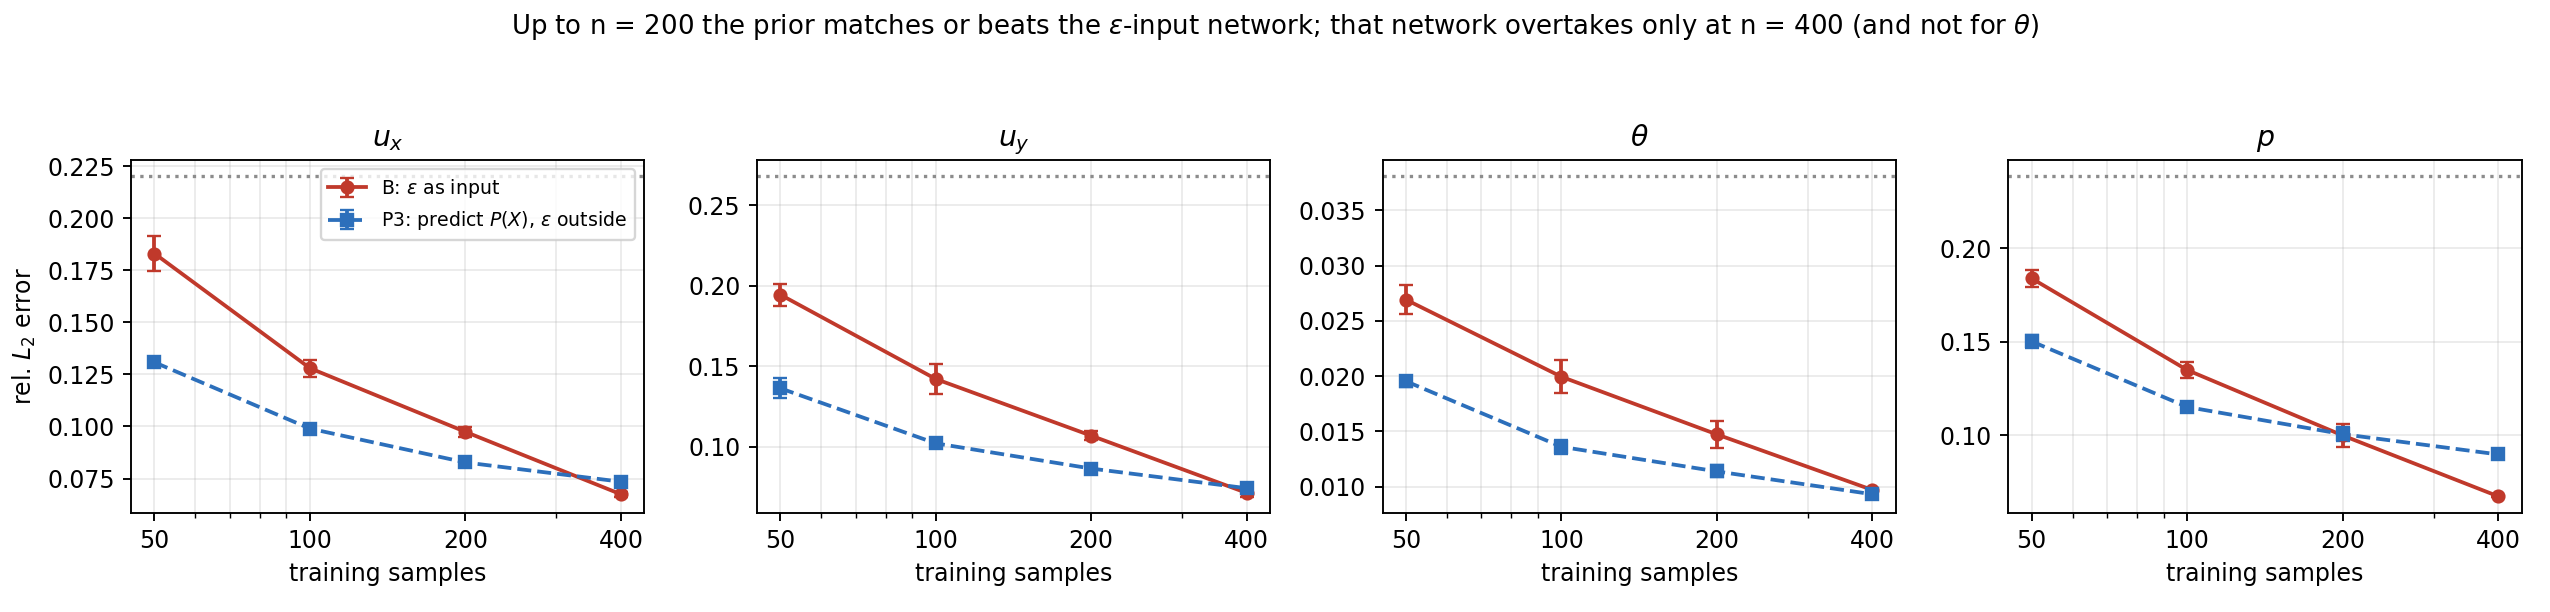
\includegraphics[width=0.98\textwidth]{fig4_learning.png}
\caption{Learning curves. Up to $n=200$ the prior matches or beats the $\varepsilon$-input network;
the latter overtakes only at $n=400$, and not for $\theta$.}
\label{fig:learning}
\end{figure}

The naive expectation---that a structured model trades in-distribution accuracy for
extrapolation---is wrong at small $n$. At $n=50$ the prior is $1.4\times$ better than the
$\varepsilon$-input network ($u_x$ 0.1308 against 0.1831, a $9\sigma$ separation across three seeds),
and it is still ahead at $n=200$ in $u_x$ ($7.3\sigma$), $u_y$ ($7.6\sigma$) and $\theta$
($3.6\sigma$), with $p$ already level ($0.13\sigma$) there. The crossover sits between $n=200$ and
400 in $u_x$ and $u_y$ (log-linear interpolation: $n\approx315$ and 360, i.e.\ near 300 in $u_x$),
essentially at $n=200$ in $p$, and $\theta$ never crosses---at $n=400$ it is still $2.5\sigma$
behind. Concretely, the prior at $n=200$ reaches what the $\varepsilon$-input network needs
$\approx270$ samples ($u_x$) and 290 ($u_y$) to reach. So the prior is two things at once: the
cheaper model when data is scarce, and---a model that needs no
$\varepsilon$ in its input, which is what makes a single-$\varepsilon$ data set reusable.

\subsection{External validation on an independent, published data set}
\label{sec:public}

\path{NurshatMenglik/NeuralConvection_2D_TrainTest} (v2; 4000 training pairs plus 200
in-distribution test pairs, CC BY 4.0), generated by another group with their own pipeline, at a
single $\varepsilon=1.2$, $Ra\in[10^2,3\cdot10^6]$ \citep{menglik2026neural}.

\paragraph{Conventions match} Recomputing their published \path{relL2_*} columns as
$\|Y-X\|/\|X\|$ from the tensors reproduces them exactly (0.14233/0.13749/0.01356/0.19070 for
sample 0); their pressure amplitude ratio is 0.929 against 0.960 for our fixed pairing, under the same
median convention.

\paragraph{The law reproduces} On the $\varepsilon=1.2$ slice:

\begin{table}[htbp]
\centering
\small
\caption{External validation at $\varepsilon=1.2$: public data against our own slice. Medians with
p10--p90 in parentheses.}
\label{tab:public}
\begin{tabular}{@{}lcc@{}}
\toprule
channel & public 4000 (median, p10--p90) & our data at $\varepsilon\in[1.1,1.3]$ ($n=64$)\\
\midrule
$u_x$ & 0.1797 (0.112--0.300) & 0.1839 (0.126--0.284)\\
$u_y$ & 0.2435 (0.141--0.403) & 0.2250 (0.150--0.395)\\
$\theta$ & 0.0228 (0.001--0.071) & 0.0232 (0.001--0.056)\\
$p$ & 0.1858 (0.117--0.246) & 0.1889 (0.128--0.262)\\
\bottomrule
\end{tabular}
\end{table}

\paragraph{Even the secondary trends reproduce} The correlation of $R$ with $\log_{10}Ra$ is
$+0.133/-0.419/+0.647/-0.198$ on their $\varepsilon\equiv1.2$ data and
$+0.032/-0.511/+0.662/-0.263$ on our $\varepsilon\in[1.1,1.3]$ slice (64 samples,
$u_x/u_y/\theta/p$). The $\theta$ channel---the one whose scatter we explain next---has $r=+0.66$ on
ours and $+0.65$ on theirs, from independently generated data.

\paragraph{Five splits, four prefactors, one predictable pattern} The release publishes three
further held-out splits generated by the same generator and the same solver commit
(\path{v6_freefall_20260921}, \path{raw_both_deramp} pressure convention; the OOD split
carries the later tag \path{v6_freefall_ood_20260925}): \path{test_in_distribution} (200
random-wall pairs), \path{test_ood} (200 random-wall pairs whose vertical-wall Fourier dials lie
outside the training range) and \path{test_legacy} (200 pairs of the classical cavity: constant
hot and cold side walls, adiabatic top and bottom). We had already downloaded
\path{train_legacy}, 5000 classical-cavity pairs. Recomputing all of \path{relL2_u_x},
\path{relL2_u_y}, \path{relL2_T}, \path{relL2_p} for every sample of all five
splits (38\,400 values: 9600 samples $\times$ 4 channels) under our conventions reproduces the
published numbers to within $1.2\times10^{-7}$ (float32 round-off;
\path{code/verify_conventions.py}), so nothing below is a convention artefact. At the fixed
$\varepsilon=1.2$ the medians of $R=\|Y-X\|/\|Y\|$ are listed in Table~S5 of the supplementary
material for all five splits, and in Table~\ref{tab:public} for the two that matter here.



The exponent cannot be re-tested here---every split sits at one $\varepsilon$---but the prefactor is
put under pressure and it moves: by $1.66\times$ ($u_x$), $1.38\times$ ($u_y$), $4.05\times$
($\theta$) and $1.07\times$ ($p$) between the classical cavity and the random-wall families at the
same $\varepsilon$, and \path{train_legacy} and \path{test_legacy} agree to three digits in
$u_x$ and $p$ ($\theta$: 0.0926 vs 0.0836, 10\%), which is the internal consistency check for the
whole comparison. That is a statement about the flow, not a defect of the law, and the $\theta$
channel makes the mechanism explicit. Writing $\hat u=\max\|\bm u_X\|$ for the peak speed of the Boussinesq field, which is available to
any surrogate, the $\theta$-channel prefactor collapses on $\hat u$ (Fig.~\ref{fig:theta}); the
fits are in Table~S6 of the supplementary material.



\begin{figure}[htbp]
\centering
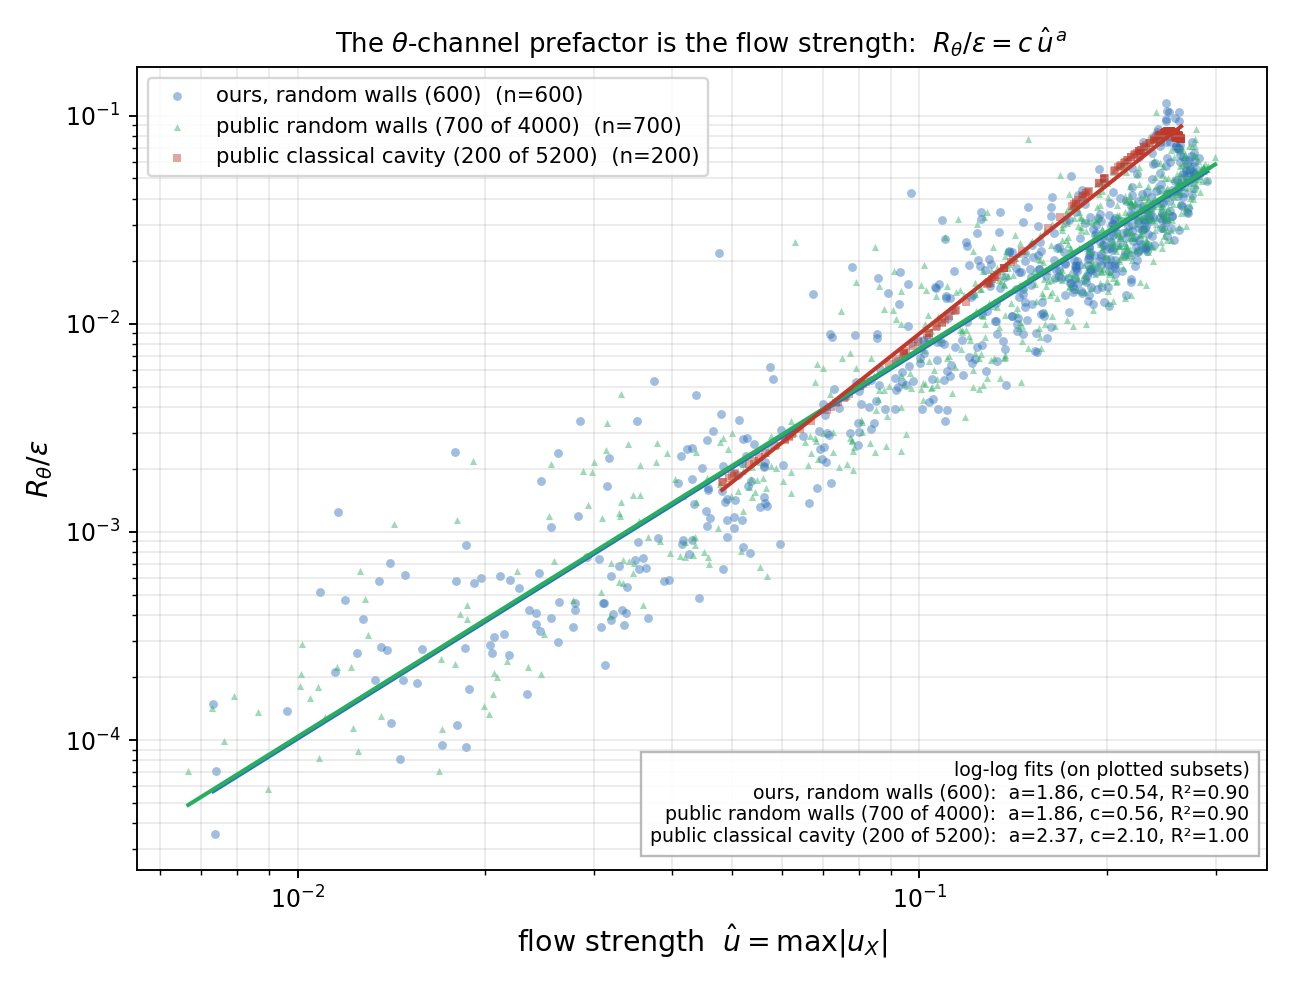
\includegraphics[width=0.78\textwidth]{fig7_theta_flow.png}
\caption{The $\theta$-channel prefactor collapses on the peak Boussinesq speed $\hat u$ across two
independent generators and two boundary-condition families.}
\label{fig:theta}
\end{figure}

Two independent groups, two independent generators, six data sets: the random-wall families all give
$c=0.54$--$0.69$, the classical cavity---whose flow is a single strong circulation with $\hat u$
41\% above the public random-wall median and 56\% above ours---gives $c=2.06$--$2.10$
(\path{code/exp_uhat_law.py}). The same reading explains the residual scatter in $u_x/u_y/p$ in
Sec.~\ref{sec:law}: $A$ is a functional of the flow, and the flow is in the input.
\subsection{What the correction does to the wall heat transfer}
\label{sec:nu}

Every error quoted so far is a field error. For a heat-transfer application the quantity that
matters is the Nusselt number, and the public classical cavity answers the question directly at
$\varepsilon=1.2$, because the two members share mesh and boundary conditions. We compute
$Nu=-\langle\partial\theta/\partial n\rangle$ at the hot wall with a six-point one-sided stencil.
On the Boussinesq member the same flux can be obtained without any wall stencil, from the
horizontally integrated flux $\int[u_x\theta-(Ra\,Pr)^{-1/2}\partial_x\theta]\,dy$, which is
independent of $x$ to $0.1\%$ at the three interior planes $x=0.25,0.5,0.75$; the wall estimate
agrees with it to $0.35\%$, which indicates the discretisation error of the estimator.

\begin{table}[htbp]
\centering
\footnotesize
\setlength{\tabcolsep}{4pt}
\caption{Wall heat transfer at $\varepsilon=1.2$ over the 200 classical-cavity samples of the
public data set. The local change is $\Delta Nu(y)/Nu(y)$ along the hot wall. The integral change is
the mean of the per-sample ratios at the six-point stencil, with the median and the 10--90\% range;
the ratio of the ensemble means is $+0.67\%$. The stencil range is the two- to eight-point
one-sided estimate of the wall gradient.}
\label{tab:nu}
\begin{tabular}{@{}p{4.4cm}p{2.5cm}p{5.2cm}@{}}
\toprule
quantity & value & spread over samples\\
\midrule
$Nu$, Boussinesq $X$ & 3.514 & ---\\
$Nu$, compressible $Y$ & 3.538 & ---\\
integral change $\Delta Nu/Nu$ & $+0.54\%$ & median $+0.58\%$, p10--p90 $+0.06$ to $+0.92\%$; per-sample mean $+0.35$ to $+0.62\%$ over stencils\\
local change, $L_1$ norm over the wall & $4.25\%$ & p90 $7.33\%$; unchanged for two to eight points\\
local change, pointwise & $-0.65\%$ (median) & p10--p90 $-9.1$ to $+9.8\%$\\
\bottomrule
\end{tabular}
\end{table}

\begin{figure}[htbp]
\centering
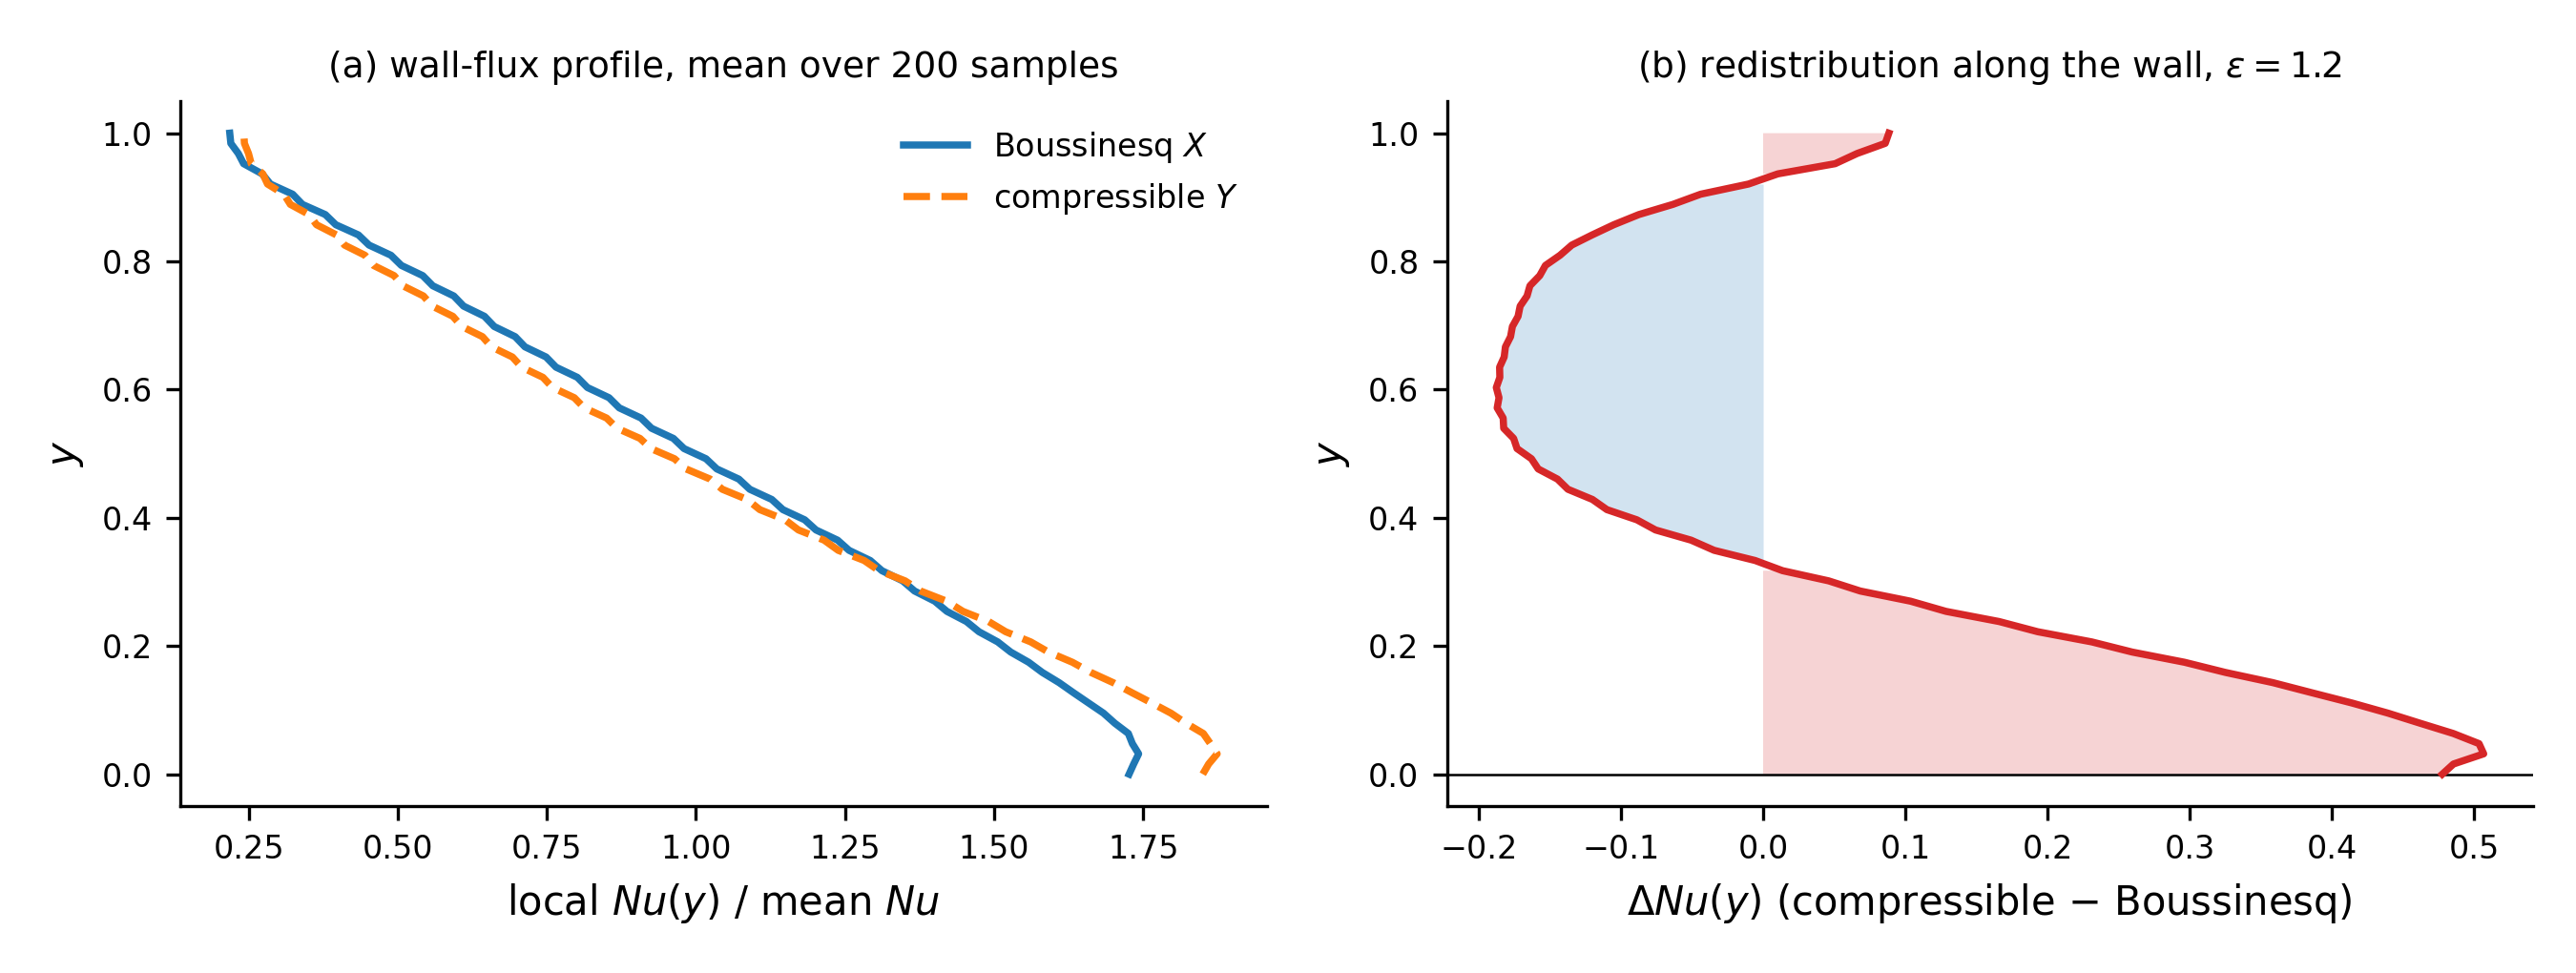
\includegraphics[width=1.0\textwidth]{fig_wallflux.png}
\caption{Wall heat transfer of the pair at $\varepsilon=1.2$. (a) Local Nusselt number along the
hot wall, normalised by its mean, for the two members. (b) Redistribution along the wall: the
compressible member carries more heat in the lower half and less in the upper half, while the
integral changes by less than $1\%$.}
\label{fig:wallflux}
\end{figure}

The two statements are different in kind. The integral heat transfer is insensitive: the
compressible member carries more heat in all 200 samples, by $0.01$--$0.94\%$ (median $0.58\%$,
10--90\% range $0.06$--$0.92\%$). The $+0.54\%$ of Table~\ref{tab:nu} is the mean of the per-sample ratios at the six-point
stencil, and the ratio of the ensemble means is $+0.67\%$. Across two- to eight-point stencils the
per-sample mean spans $+0.35$ to $+0.62\%$ and the ratio of the ensemble means $+0.30$ to
$+0.90\%$. The local wall flux is not: the correction redistributes
it by $4.25\%$ in $L_1$ (p90 $7.33\%$), with pointwise excursions of $\pm10\%$, and that number is
the same for every stencil order. On average the correction adds heat over the lower half of the
cavity and removes it over the upper half (Fig.~\ref{fig:wallflux}b); the integral is the
$Nu$-weighted mean of this redistribution, which is why it cancels. A surrogate trained on
Boussinesq data therefore predicts the total heat load to better than $1\%$ at this contrast and
the local flux to only about $4\%$; which of the two matters is set by the application, not by the
physics. The field statistic behind the cancellation is large: on the same 200 samples the
temperature field itself differs by $8.4\%$ in relative $L_2$, so an $8.4\%$ change in the field
produces a $0.6\%$ change in its wall-normal derivative.

The gap grows with contrast. On the 20 configurations that carry five contrasts the mean of the per-sample
relative gaps is $+0.11\%$ at $\varepsilon=0.4$, $+0.44\%$ at 0.8, $+1.09\%$ at 1.2, $+2.42\%$ at
1.6 and $+5.06\%$ at 1.9, a log--log slope of 2.4; individual flows scatter around it (at
$\varepsilon=1.9$ the 10--90\% range is $-6.1$ to $+23\%$), because the sign of the local
redistribution differs between flows. The heat load is therefore a second-order effect that
reaches $5\%$ only near $\varepsilon=2$, but it is not zero, and a Boussinesq-trained surrogate
cannot produce it: the three-orders-of-magnitude saving over the compressible solve is bought by
keeping the compressible correction, not by replacing it with a cheaper Boussinesq run.

\subsection{Cross-data-set transfer: the payoff, and its boundary}
\label{sec:transfer}

Two public single-$\varepsilon$ data sets are available (Table~\ref{tab:transfer},
Fig.~\ref{fig:transfer}): 4000 random-wall pairs (our
boundary-condition family) and 5000 classical-cavity pairs (a different one). Both sit at
$\varepsilon\equiv1.2$. We train the same U-Net on each---once with the plain output (target $D$),
once with the prior (target $D/\varepsilon$, and $\varepsilon$ multiplied back outside the
network)---and apply the result to our own 600 samples with no retraining, at
$\varepsilon$ from 0.2 to 1.9, values the training data never contained.

\begin{table}[htbp]
\centering
\footnotesize
\setlength{\tabcolsep}{4pt}
\caption{Transfer from a single-$\varepsilon$ public data set to our own
$\varepsilon\in[0.2,1.9]$ samples, on the extrapolation and interpolation test splits. Entries are
$u_x/u_y/\theta/p$. The last row uses 382 training samples for the extrapolation column and 400
for the interpolation one. Both public sets are at $\varepsilon\equiv1.2$. That row is the $\varepsilon$-blind prior (no $\varepsilon$ input, 150
epochs, one seed), the same protocol as the public rows above; the P1/P3 columns of
Table~\ref{tab:ablation} use 200 epochs and three seeds.}
\label{tab:transfer}
\setlength{\tabcolsep}{3pt}
\begin{tabular}{@{}p{3.9cm}p{0.8cm}p{3.75cm}p{3.75cm}@{}}
\toprule
trained on & model & extrapolation ($n=218$) & interpolation ($n=200$)\\
\midrule
do nothing & $\hat Y=X$ & 0.3018/0.3731/0.0556/0.3320 & 0.2203/0.2683/0.0381/0.2386\\
public 4000, random walls & plain &
0.1443/0.1730/0.0226/0.1838 & 0.1199/0.1441/0.0189/0.1435\\
public 4000, random walls & prior &
0.0932/0.1085/0.0119/0.1322 & 0.0657/0.0769/0.0077/0.0891\\
our own training split & prior & 0.1250/0.1321/0.0170/0.1719 & 0.0791/0.0811/0.0103/0.0947\\
public 5000, classical cavity & plain &
0.2919/0.3711/0.0490/0.3192 & 0.2444/0.3612/0.0484/0.3217\\
public 5000, classical cavity & prior &
0.3092/0.4730/0.0561/0.3280 & 0.2281/0.3498/0.0422/0.2584\\
\bottomrule
\end{tabular}
\end{table}

\begin{figure}[htbp]
\centering
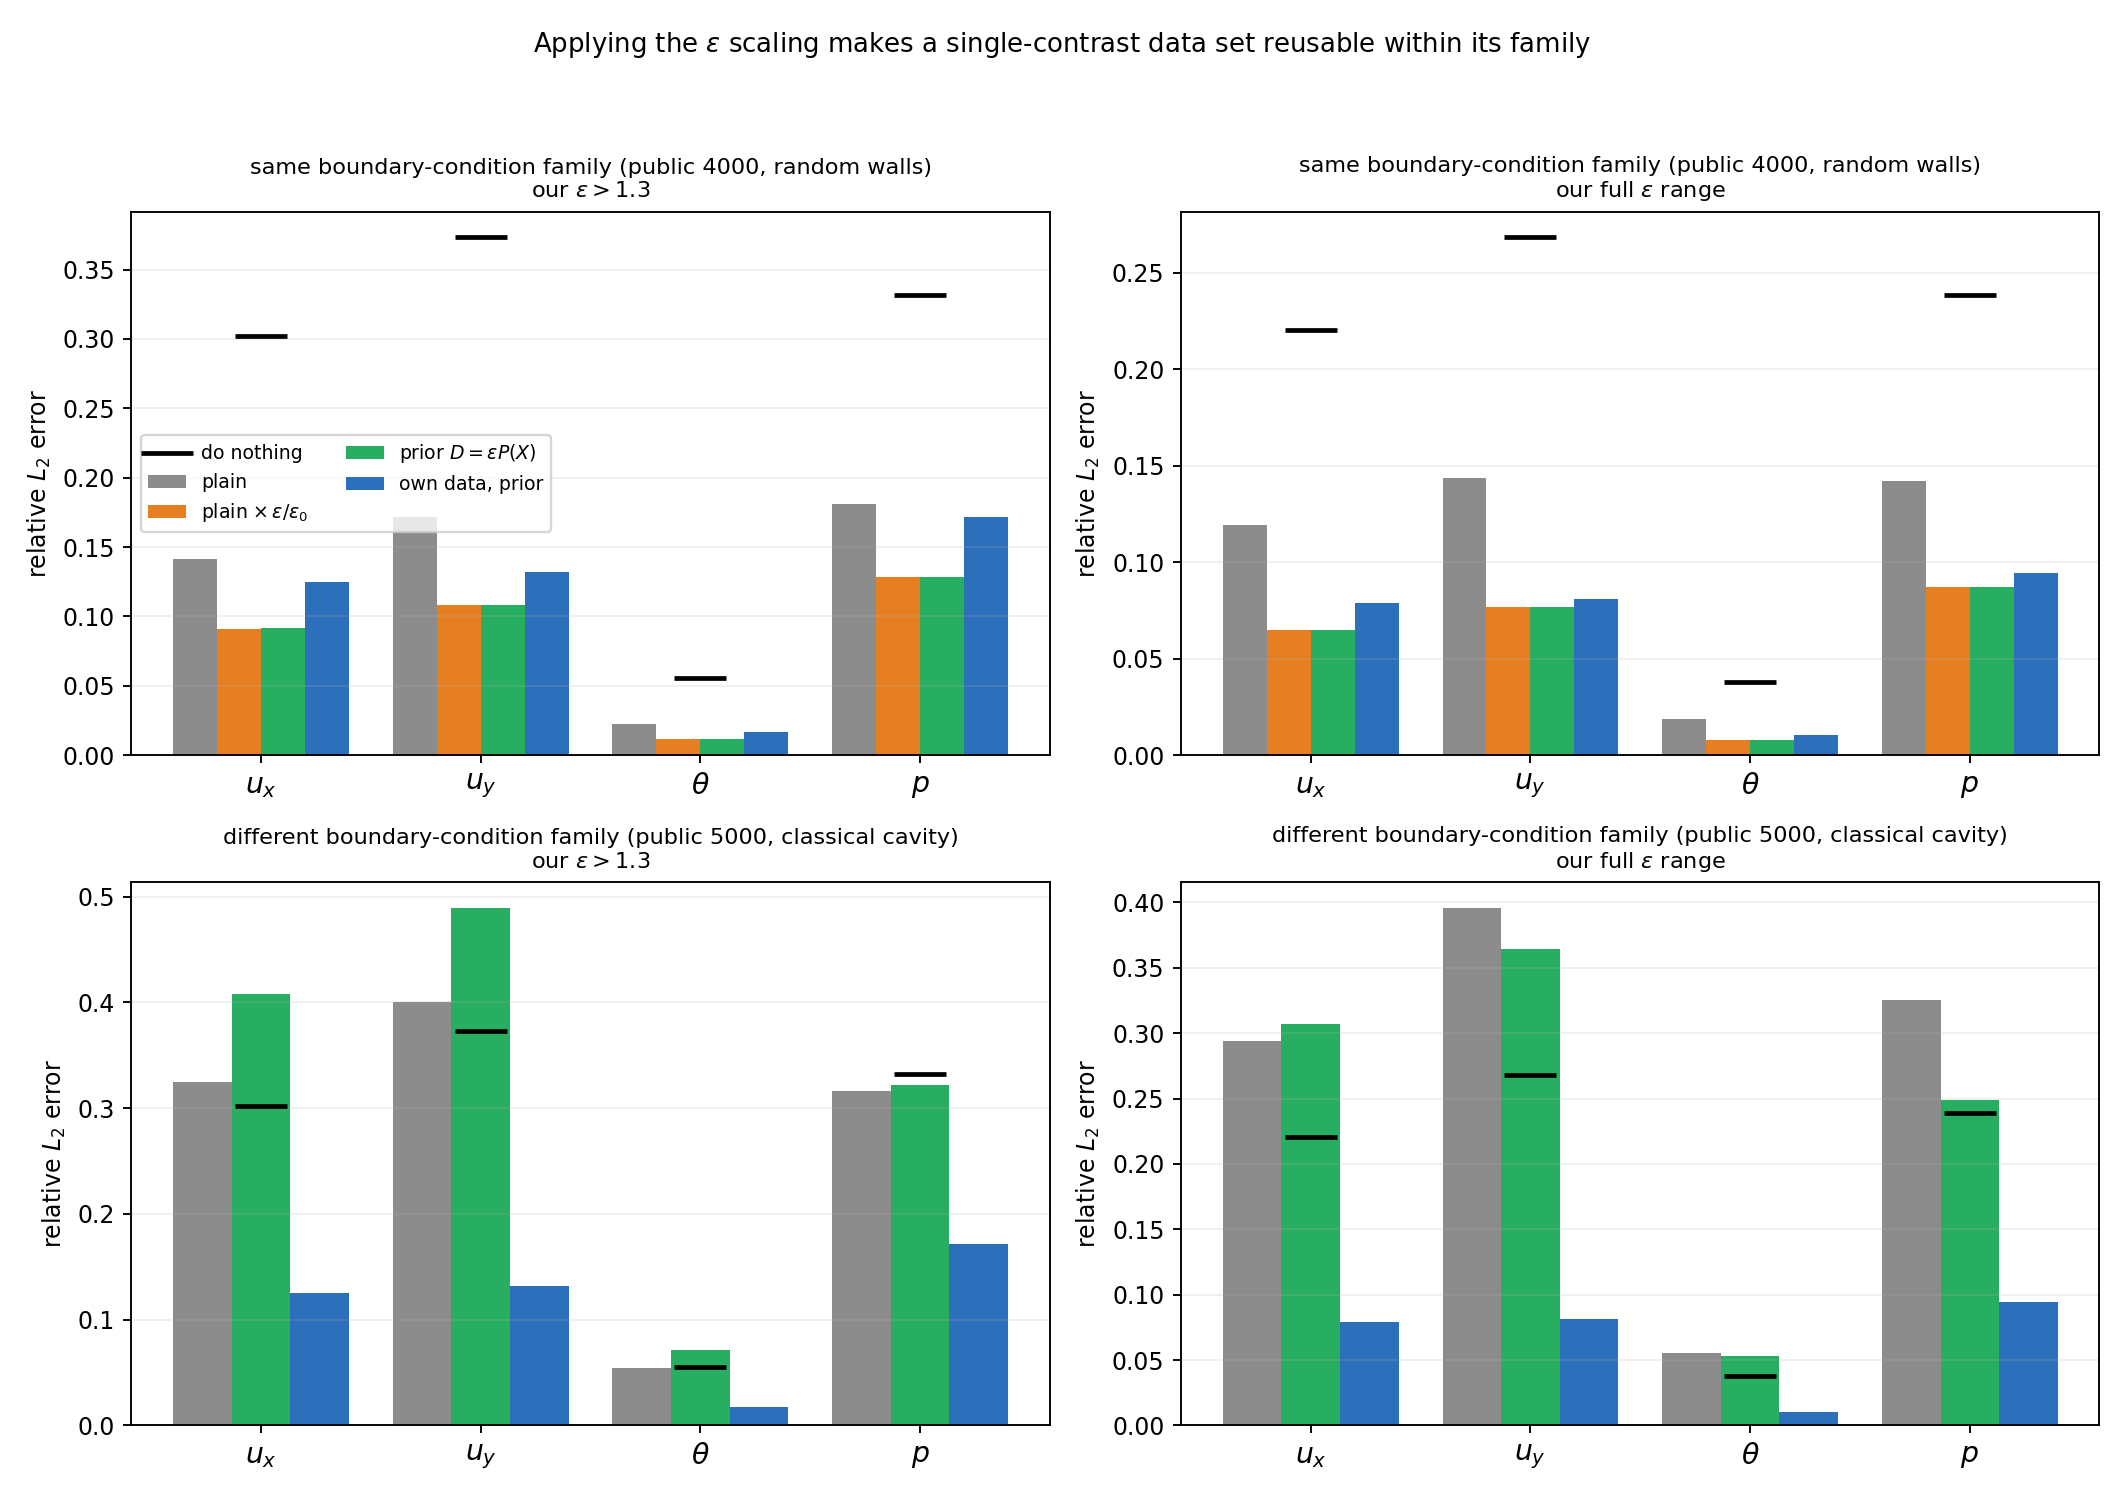
\includegraphics[width=0.9\textwidth]{fig6_transfer.png}
\caption{Reusing a single-$\varepsilon$ data set. Within the boundary-condition family the prior
transfers and beats the plain model; across families it fails, and can be worse than doing
nothing.}
\label{fig:transfer}
\end{figure}

Three readings, in order of how much they matter for practice.

\begin{itemize}
\item Within the family, the prior is what makes a single-$\varepsilon$ data set reusable.
The identical architecture, budget and data give 0.1443 ($u_x$) with the plain output and 0.0932
with the prior---a factor 1.55---and $3.2\times$ better than doing nothing, on $\varepsilon$ the
data never contained. It is even better than the same prior trained on our own 382 samples
(0.1250), because it sees ten times more configurations. This is the concrete content of ``the
$\varepsilon$ dependence need not be in the data''.
\item The prior also fixes the failure mode of the plain model. The plain model's error at
unseen $\varepsilon$ is largest where the training $\varepsilon$ is furthest away (its correction
is a fixed field, Sec.~\ref{sec:floor}), whereas the prior's error stays proportional to how wrong
$P$ is, uniformly in $\varepsilon$.
\item Across boundary-condition families the same trick fails, and the prior makes it
worse. Trained on the classical cavity, the plain model lands at 0.2919 against a floor of
0.3018---it learned almost nothing transferable---and the prior model is \emph{worse} than the
plain one (0.3092 at $\varepsilon>1.3$): it confidently multiplies a $P$ learnt on the wrong flow by
an $\varepsilon$ that grows to 1.9. This is exactly what Sec.~\ref{sec:public} predicts, and it is
the same number: $A$ is a functional of the flow, the classical cavity's flow has $\hat u$ 41\%
above the random-wall median, and a surrogate trained on that family predicts the wrong $A$.
Reusing published data therefore requires the boundary-condition family to be represented; the law
tells you in advance which reuse will work (\path{code/exp_public_transfer.py},
\path{code/exp_public_legacy_transfer.py}).
\end{itemize}

\subsection{A second geometry (aspect ratio 2:1, 104 samples)}
\label{sec:aspect}

Same generator, same $Ra$ and $\varepsilon$ ranges, cavity twice as wide (Fig.~\ref{fig:axes}).
The $\varepsilon$ exponent is unchanged in the $\varepsilon$-only fit ($m=1.09/1.16/0.93/1.08$ for
$u_x/u_y/\theta/p$, $0.7\sigma$, $1.8\sigma$, $0.3\sigma$ and $0.7\sigma$ away from the unit-square
values; the two-parameter values are in Table~S2), while the prefactor moves
($A=0.175/0.175/0.008/0.222$ versus $0.147/0.193/0.010/0.148$). The Rayleigh trend is stronger for
$u_x$ and $p$ here ($q=-0.14,-0.15$ vs $0.00,-0.03$) and reproduces for $u_y$ and $\theta$.
The $\varepsilon$-scaling is geometry-independent; calibration of $A$ is not---which is
exactly why the surrogate takes $X$ as input rather than a table of $A$. Changing the fluid instead
($Pr$ $0.71\to4.38$) moves neither the exponent nor the prefactor by more than a
few percent (Sec.~\ref{sec:water}).

\begin{figure}[htbp]
\centering
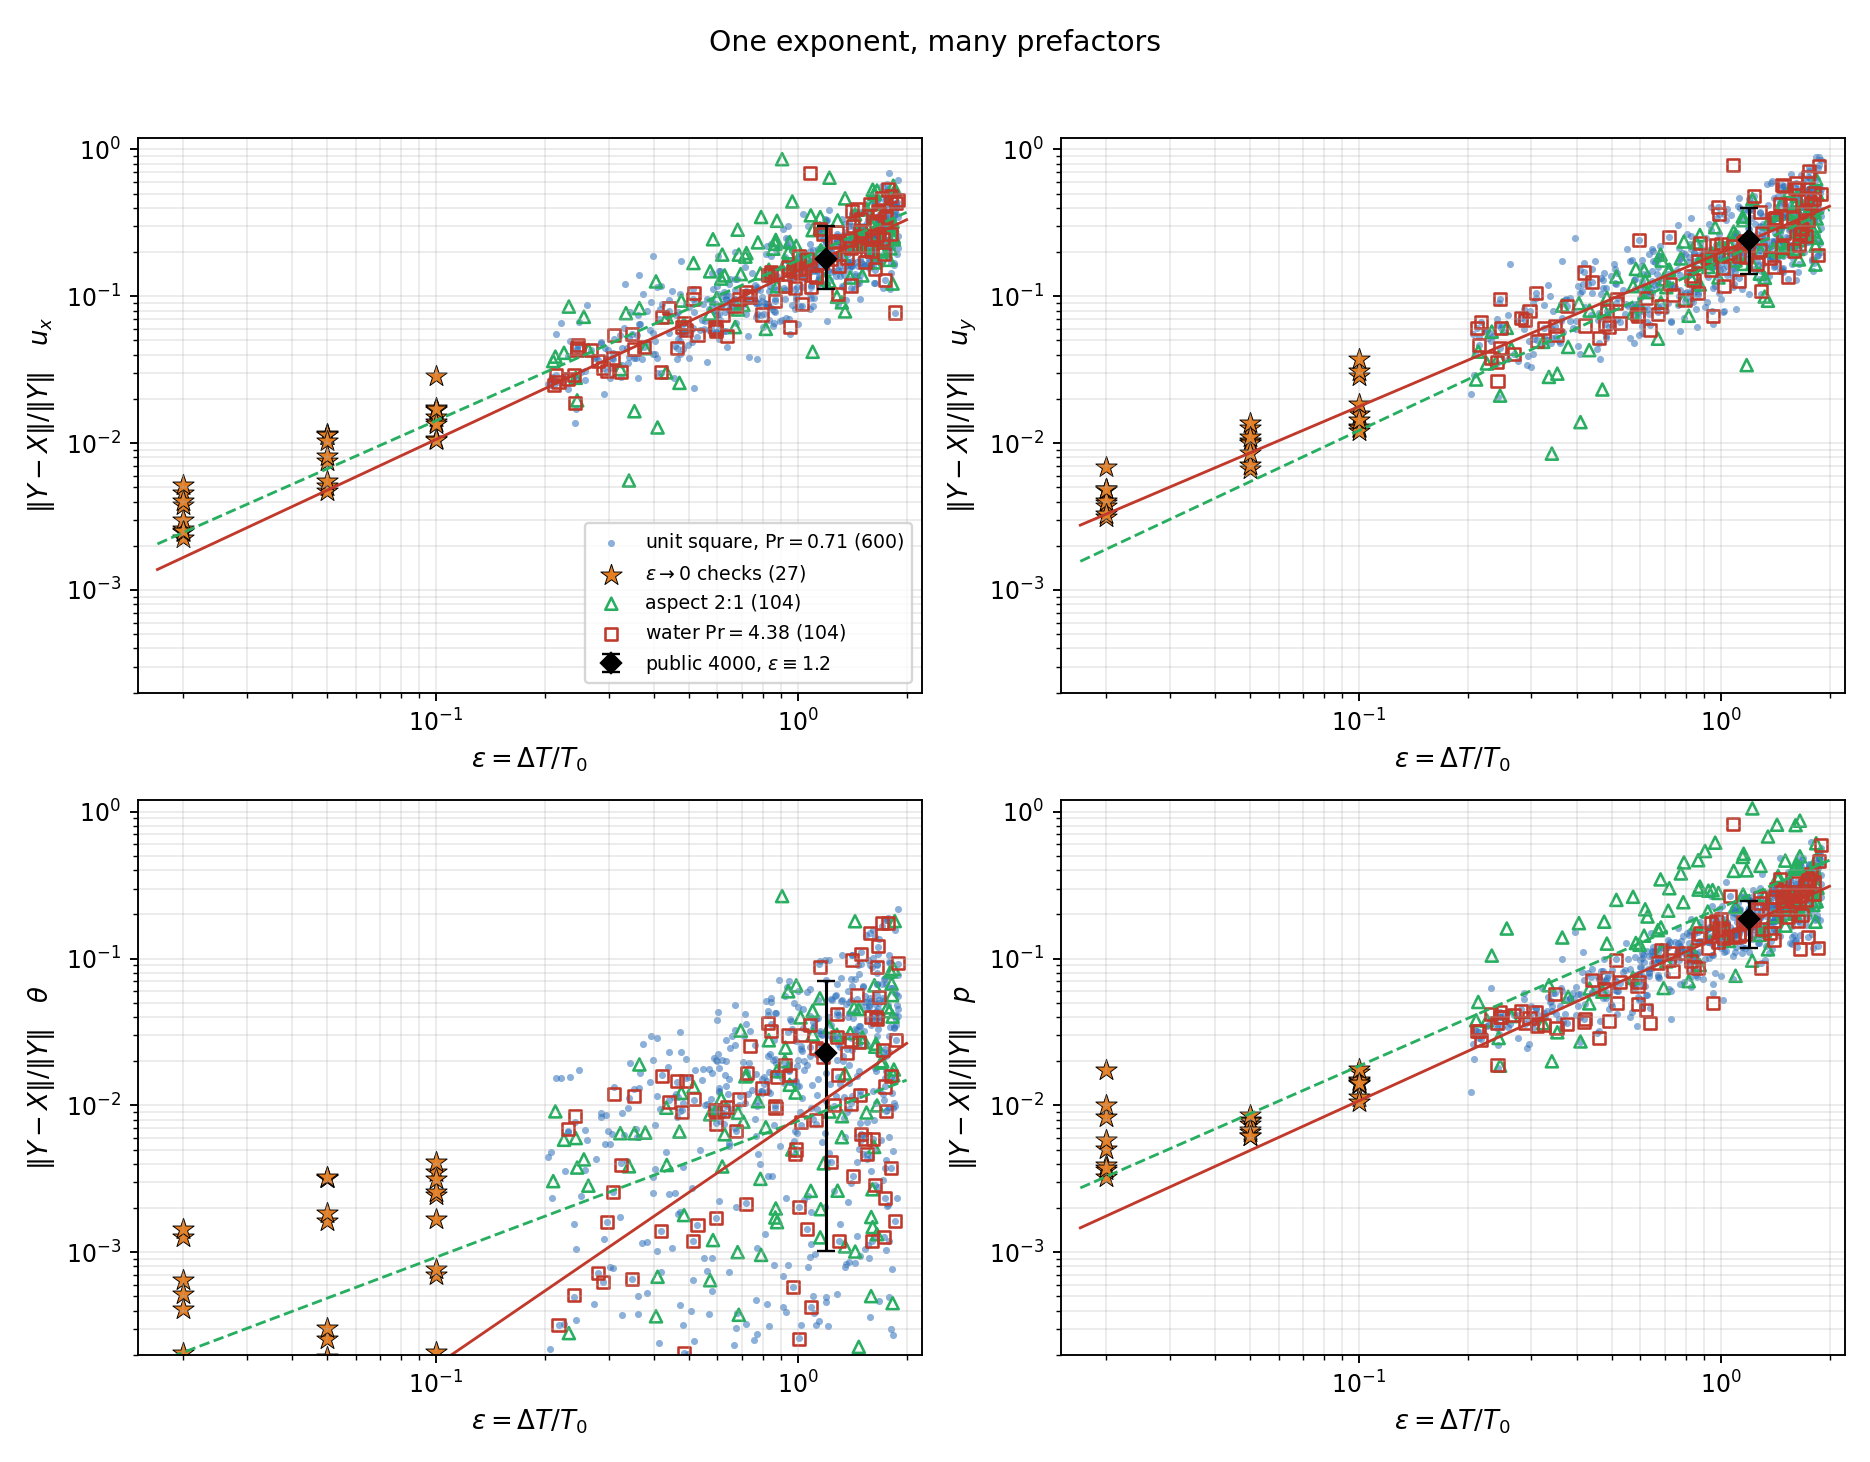
\includegraphics[width=0.95\textwidth]{fig5_law_axes.png}
\caption{One exponent, many prefactors: unit square ($Pr=0.71$), aspect 2:1, $Pr=4.38$, and the public data set at
$\varepsilon=1.2$.}
\label{fig:axes}
\end{figure}

\subsection{Solver noise is not the source of the law}
\label{sec:noise}

\begin{itemize}
\item Convergence quality over 600 samples (compressible member): median relative change
$3.75\times10^{-6}$, p90 $1.09\times10^{-4}$, worst $7.04\times10^{-4}$.
\item Dropping the 65 samples with relative change $>10^{-4}$ changes the $u_x$ fit from
$0.1809\varepsilon-0.0212$ to $0.1813\varepsilon-0.0221$---unchanged.
\item Re-running the 10 worst samples with \path{steady_tol} tightened from $10^{-6}$ to
$10^{-8}$ leaves the solution bit-identical ($|\Delta Y|/|Y|=0$). The reason is
structural: the compressible march terminates on the zero-iteration guard, not on
\path{steady_tol}, so the residual reported is the fixed-point residual of the discrete solution,
not unfinished iteration.
\end{itemize}

\subsection{Cost and speed-up}
\label{sec:cost}

\begin{table}[htbp]
\centering
\small
\caption{Wall-clock cost, $64^2$ mesh. Solver rows use eight CPU threads; the surrogate runs on
an RTX 4060 Laptop GPU (batch 1) or one CPU thread. The two members are timed separately over the
600 samples; the last two rows are totals that combine the measured medians.}
\label{tab:cost}
\begin{tabular}{@{}lcccc@{}}
\toprule
 & median & mean & p90 & max\\
\midrule
paired solve, 600 samples & 33.9\,s & 38.0\,s & 59.9\,s & 510\,s\\
Boussinesq member alone & 11.7\,s & 13.1\,s & 21.7\,s & ---\\
compressible member alone & 22.3\,s & 25.0\,s & 37.3\,s & ---\\
paired solve, 100-sample $\varepsilon$ scan & 55.8\,s & 67.7\,s & 136\,s & 202\,s\\
surrogate, GPU, batch 1 & 6.3\,ms & & &\\
surrogate, GPU, batch 256 & 0.49\,ms/sample & & &\\
surrogate, CPU, 1 thread & 14.0\,ms & & &\\
end-to-end pair (Boussinesq + surrogate) & 11.7\,s & & &\\
100-contrast sweep, total & 12.3\,s & & &\\
\bottomrule
\end{tabular}
\end{table}

Table~\ref{tab:cost} gives the wall-clock cost. A paired solve splits into a Boussinesq member
(median 11.7\,s) and a compressible member (22.3\,s); the surrogate replaces only the second. Per
pair the cost therefore falls from 33.9\,s to 11.7\,s, a factor $2.9$, and the comparison of one
inference with one compressible solve ($22.3\,\mathrm{s}/6.3\,\mathrm{ms}=3.5\times10^3$) describes only that member.
The regime that matters for a parameter study is the amortised one: $X$ does not depend on
$\varepsilon$, so $N$ contrasts cost one Boussinesq solve plus $N$ inferences. For $N=100$ that is
12.3\,s against $3.39\times10^3$\,s, a factor $2.8\times10^2$, and the Boussinesq solve is then the
limit. The solver runs on eight CPU threads and the surrogate on a GPU; the two are not the same
hardware.

\subsection{A third Prandtl number: $Pr=4.38$}
\label{sec:water}

$Pr$ and $\varepsilon$ do not mix. $Pr$ enters the coefficients of both members
($Re^{-1}=(Pr/Ra)^{1/2}$) and hence the Boussinesq solution $X$, but the $\varepsilon$-expansion of
Sec.~\ref{sec:theory} never multiplies the two. The prediction is therefore sharp and asymmetric:
the exponent must not move, while the prefactor may, because $X$ itself has changed.

We generated 104 further pairs at $Pr=4.38$, the Prandtl number of water near $40^\circ$C, keeping
the equation of state, $\gamma$ and the transport coefficients of the air run: the study isolates
the $Pr$ axis and does not claim water properties (Table~\ref{tab:water}, Fig.~\ref{fig:water}).
The pairs are bit-identical to
the first 104 samples of the main batch in every other respect: same seed stream, hence the same
wall-temperature Fourier draws, the same $Ra$ and the same $\varepsilon$. The two families are
therefore a strict paired experiment in which the fluid is the only difference (the Mach-number law
is unchanged, and $Ma$ is inert, Sec.~\ref{sec:axis}).

\begin{table}[htbp]
\centering
\footnotesize
\setlength{\tabcolsep}{3pt}
\caption{The fluid axis: 104 strictly paired configurations at $Pr=0.71$ and $Pr=4.38$ (same seed
stream, same $Ra$ and $\varepsilon$). The exponent is unchanged; the paired median ratio of $R$ is
0.95--1.01, while the fitted prefactor of $\theta$ moves by 15\% because the fit re-weights the
ensemble.}
\label{tab:water}
\begin{tabular}{@{}lcccc@{}}
\toprule
channel & $A$, $Pr=0.71$ & $A$, $Pr=4.38$ & $m$, $Pr=0.71$ & $m$, $Pr=4.38$\\
\midrule
$u_x$ & 0.1468 & 0.1496 & $1.157$ & $1.150$\\
$u_y$ & 0.1934 & 0.1985 & $1.047$ & $1.049$\\
$\theta$ & 0.0097 & 0.0082 & $1.668$ & $1.686$\\
$p$ & 0.1482 & 0.1426 & $1.109$ & $1.124$\\
\bottomrule
\end{tabular}
\end{table}

\begin{figure}[htbp]
\centering
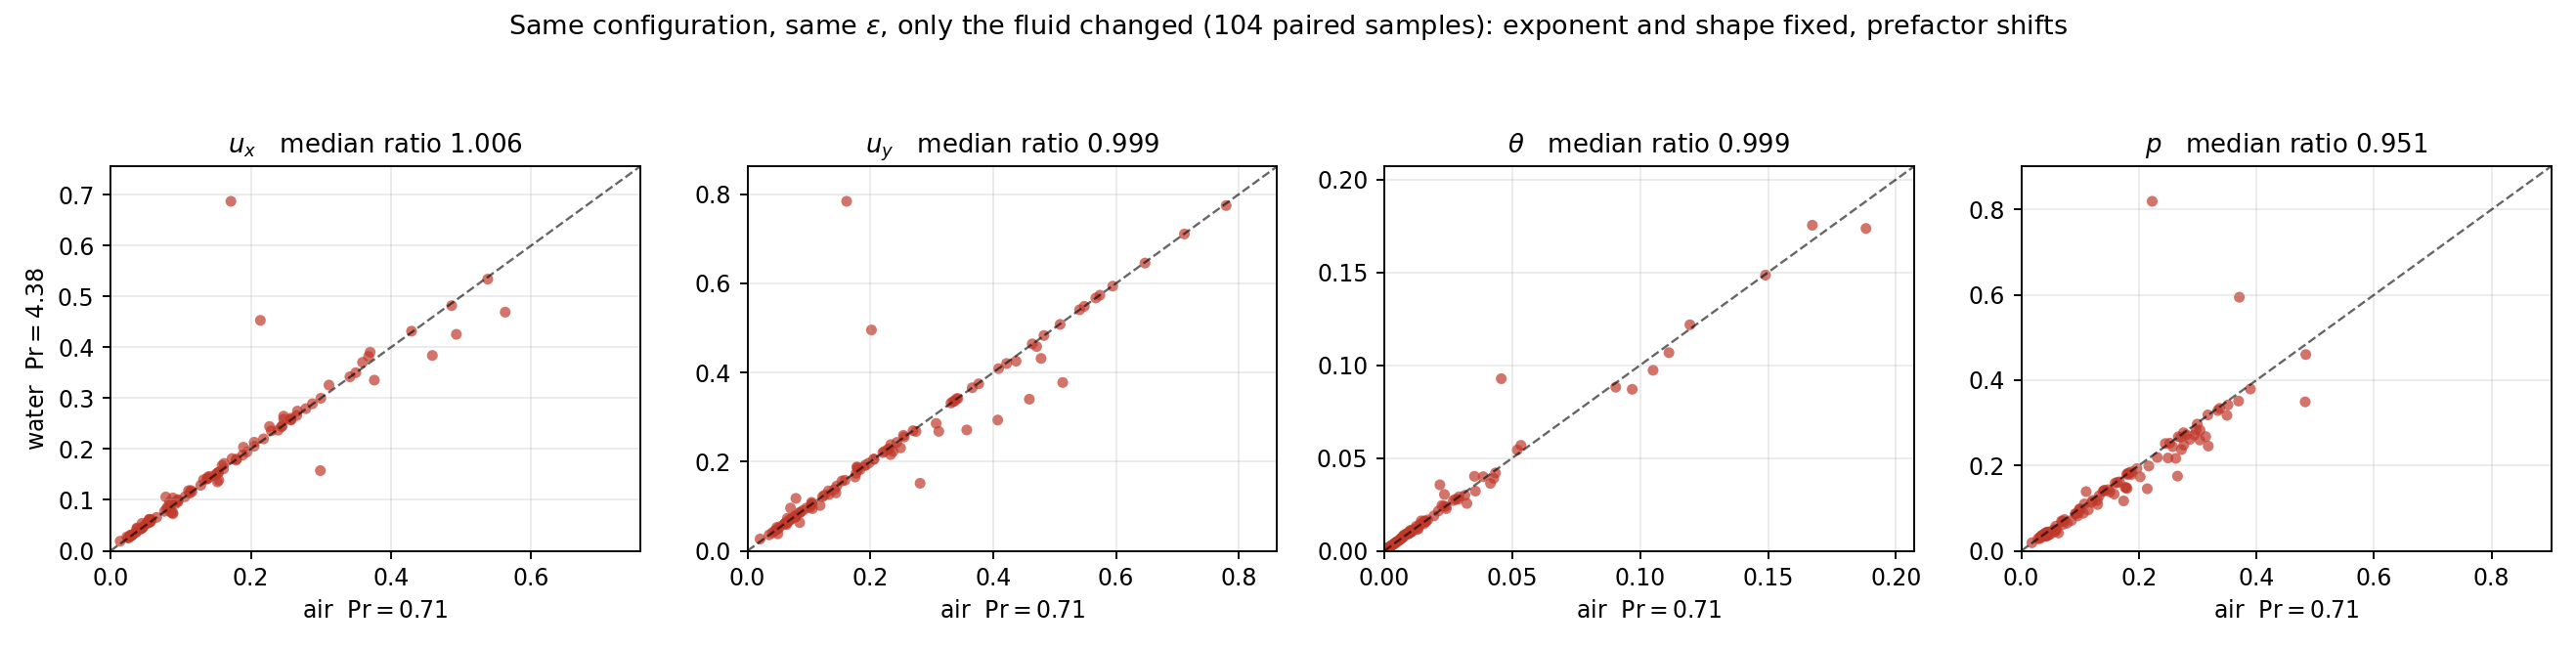
\includegraphics[width=0.96\textwidth]{fig8_water.png}
\caption{Same configuration, same $\varepsilon$, only the Prandtl number changed: $Pr=0.71$ against
$Pr=4.38$, 104 paired samples. The panel labels follow the original run names; both runs use the
same equation of state and transport coefficients, and only $Pr$ differs.}
\label{fig:water}
\end{figure}

On the 104 matched configurations the paired ratios $R(Pr=4.38)/R(Pr=0.71)$ have
medians 1.006, 0.999, 0.999 and 0.951 ($u_x/u_y/\theta/p$; p10--p90
0.99--1.12, 0.90--1.03, 0.95--1.06, 0.82--1.00), and the paired exponents agree to $1$--$2\%$:
$1.150$ vs $1.157$, $1.049$ vs $1.047$, $1.686$ vs $1.668$, $1.124$ vs $1.109$. A 6.2-fold change
in Prandtl number leaves the discrepancy of the same configuration unchanged to $0.1\%$ in
$\theta$, $0.1\%$ in $u_x$ and $u_y$, and $5\%$ in $p$.

$Pr$ is therefore not a break-symmetry axis either, and the law's two ingredients separate
cleanly: $\varepsilon$ sets the exponent, the flow sets the prefactor, and the fluid changes neither
by more than a few percent on the paired comparison. Keeping
the strict pairing matters for the last digit---the unpaired fits give $\theta$ $0.0097\to0.0082$
(a 15\% move, the same direction as the 5\% paired move) and $u_x/u_y$ $+2$--3\%---which is the same
statement as Sec.~\ref{sec:aspect} (a geometry moves $A$) and Sec.~\ref{sec:public}
(boundary-condition families move it by up to $4\times$).
\subsection{A three-dimensional check}
\label{sec:3d}

The law is calibrated in two dimensions. To test whether the exponent survives in three, we
generated twelve paired steady solutions with the same generator: three fixed flows---a three-cell
Voronoi wall pair, a two-cell wall pair and a constant-wall cavity---each solved at
$\varepsilon=0.2$, $0.4$, $0.8$ and $1.2$, with $Ra=10^4$, $Pr=0.71$ and $res=16$ ($33^3$ velocity nodes,
$17^3$ temperature and pressure nodes). The pairing is exact: within each flow the wall temperatures
are the same seed stream scaled affinely about $T_0$, so the low-fidelity member is the same
solution up to the $\varepsilon$-blind rescaling of Sec.~\ref{sec:blind}.

Table~\ref{tab:3d} and Fig.~\ref{fig:3d} give the result. In every channel and every flow a
power law fits the four $\varepsilon$ values in log--log coordinates with $R^2>0.998$, and the per-flow exponents are
$1.063\pm0.019$ ($u_x$), $1.033\pm0.012$ ($u_y$), $1.092\pm0.015$ ($\theta$) and
$1.100\pm0.010$ ($p$)---within $0.11$ of unity and the flow-mean exponents within $0.10$ of the two-dimensional
full-window fit of Table~\ref{tab:law}. The comparison is to the full-window fit rather than to a
2-D fit restricted to the same window: the 2-D samples are drawn at random $\varepsilon$ and their
prefactor varies by up to $4\times$ between flows (Sec.~\ref{sec:public}), so a narrow-window
regression there measures that scatter rather than the local slope. The prefactor is not universal here either: across the three flows it varies
by $3.8\times$ ($u_x$), $2.0\times$ ($u_y$), $10\times$ ($\theta$) and $2.0\times$ ($p$), which is
the same statement as Sec.~\ref{sec:public}, that $A$ is a functional of the flow. What transfers to
three dimensions is the exponent, which is what the factorisation predicts.

The check is limited to $Ra=10^4$, $res=16$ and $\varepsilon\le1.2$. The twelve pairs cost
13--29\,min each (median 16\,min) of outer wall-clock time on this machine. We therefore report the exponent transfer, not
a three-dimensional sweep.

\begin{table}[htbp]
\centering
\small
\caption{Three-dimensional check: twelve strictly paired samples, three fixed flows $\times$ four
$\varepsilon$ at $Ra=10^4$, $Pr=0.71$, $res=16$. Per-flow exponents are power-law fits to the four
$\varepsilon$ values of that flow. Flows are ordered three-cell Voronoi, two-cell Voronoi, constant
wall. The prefactor is listed per flow to show that it does not transfer between flows.}
\label{tab:3d}
\begin{tabular}{@{}lccc@{}}
\toprule
channel & $m$ (mean$\pm$s.d. over flows) & per-flow $m$ & $A$ per flow\\
\midrule
$u_x$ & $1.063\pm0.019$ & 1.09/1.06/1.05 & 0.066/0.180/0.251\\
$u_y$ & $1.033\pm0.012$ & 1.04/1.02/1.04 & 0.121/0.158/0.247\\
$\theta$ & $1.092\pm0.015$ & 1.10/1.10/1.08 & 0.006/0.023/0.063\\
$p$ & $1.100\pm0.010$ & 1.10/1.11/1.09 & 0.094/0.177/0.183\\
\bottomrule
\end{tabular}
\end{table}

\begin{figure}[htbp]
\centering
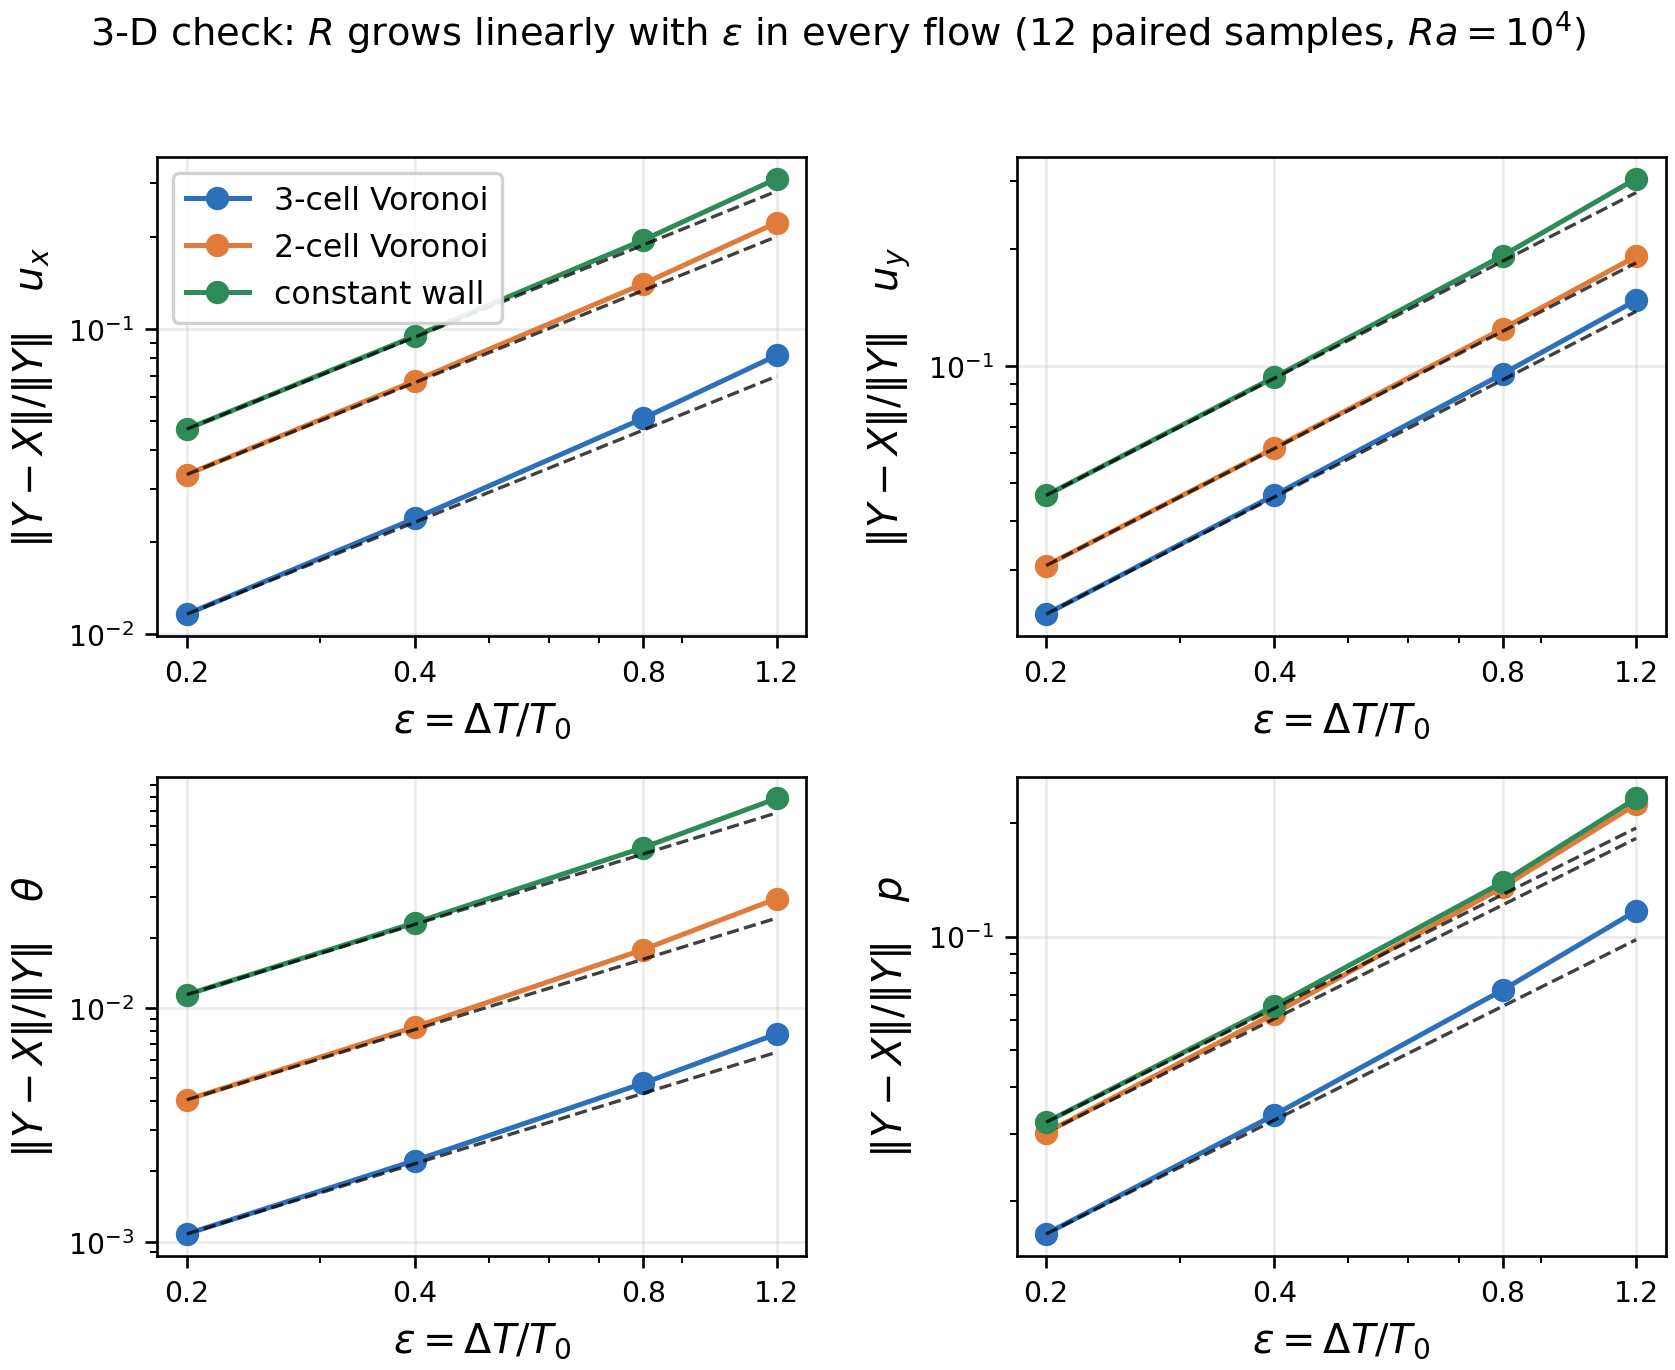
\includegraphics[width=0.95\textwidth]{fig9_3d.png}
\caption{The three-dimensional check in log--log coordinates: twelve paired samples, three fixed flows
and four temperature contrasts. Dashed lines are a slope-one reference anchored at the lowest
$\varepsilon$ of each flow.}
\label{fig:3d}
\end{figure}

\section{Limitations}
\label{sec:limits}

\begin{enumerate}
\item Two dimensions for the main sweep. The law is calibrated on 2-D solutions. The
twelve-sample 3-D check of Sec.~\ref{sec:3d} reproduces the exponent, but covers one Rayleigh number,
$res=16$ and $\varepsilon\le1.2$. Each 3-D pair costs 13--29\,min of outer wall-clock time (median 16) on this machine. A
3-D sweep at higher $Ra$ or resolution remains out of reach here.
\item $Ma$ is inert here, so the break-symmetry group is one-dimensional rather than two.
At larger $Ma$ this would have to be redone.
\item $\varepsilon<2$, imposed by the equation of state (the cold wall must stay positive).
\item The two-parameter fits of Sec.~\ref{sec:law} leave 26/23/28\% of the variance unexplained in
$u_x/u_y/\theta$ and 17\% in $p$; the $\hat u$ form of Sec.~\ref{sec:public} closes that gap for
$\theta$ and leaves the same residual flow-dependence in the other three channels.
\item The prefactor $A$ is configuration-dependent and must be learned: it moves with the geometry
(Sec.~\ref{sec:aspect}) and by $1.66\times$ ($u_x$) / $1.38\times$ ($u_y$) / $4.05\times$
($\theta$) / $1.07\times$ ($p$) between boundary-condition families of an independent data set
(Sec.~\ref{sec:public}), while it is insensitive to the fluid ($Pr$, Sec.~\ref{sec:water}).
\item The public data set and ours differ by 0.08\% in $Ra_{\mathrm{eff}}$ at $\varepsilon=1.2$
($1.2/1.095^2=1.000813$); their v2 release corrects this and the two now agree.
\end{enumerate}

\section{Conclusion}
\label{sec:conclusion}

We set out to build a surrogate for compressible natural convection and found that the object it has
to reproduce---the gap between the Boussinesq solution and the compressible one---is governed by a
single parameter in an exact and predictable way.

\begin{enumerate}
\item One parameter. In this non-dimensionalisation $Fr^2=\Delta T/T_0$ identically, so
the break-symmetry axis is $\varepsilon=\Delta T/T_0$ and nothing else; Mach-number effects are
$O(Ma^2)$ and are invisible at the values reached here.
\item A clean law. $R=\|Y-X\|/\|Y\|=A\varepsilon^m$ with
$m=1.023\pm0.018$, $0.995\pm0.019$, $1.024\pm0.077$, $1.009\pm0.015$ ($u_x,u_y,\theta,p$), an
intercept indistinguishable from zero, the exponent quoted over the full two-decade window (from
$\varepsilon=0.8$ upwards the same points give $1.23$--$1.32$, the $\varepsilon^2$ curvature of
Sec.~\ref{sec:law}), and a 134-family boundary-condition description (133 dummies) that adds only
2--3 pp of adjusted $R^2$ to the velocity and pressure channels. The exponent is
geometry-independent and fluid-independent; only the prefactor $A$ must be calibrated, which is why
the surrogate takes $X$ as input rather than a table of $A$. Twelve paired 3-D solutions reproduce
the exponent (flow means $1.03$--$1.10$, per-flow $1.02$--$1.11$; Sec.~\ref{sec:3d}).
\item A reason. The $\varepsilon$-expansion of the compressible member reproduces the
Boussinesq system at $O(1)$ and produces the correction through
$\nabla\cdot\bm u_1=\nabla\cdot(\theta_0\bm u_0)$ and the density-modulated inertia. The linearised
operator does not contain $\varepsilon$, so the correction factorises,
$D=\varepsilon P(X)+\varepsilon^2Q(X)+\dots$, with a shape that does not rotate. All five
consequences of the expansion are confirmed numerically.
\item A design rule. Predicting $P(X)$ and multiplying by $\varepsilon$ outside the
network---two lines of code---converts the law into a prior that (i) beats the plain architecture
by $1.07$--$1.15\times$ over a FiLM-conditioned network, (ii) lets the network discover the $\varepsilon^2$ term itself,
(iii) works the same way for a Fourier neural operator, and (iv) makes a public data set that exists
at a single temperature contrast reusable at others---0.093 ($u_x$) on $\varepsilon>1.3$ against
0.144 for the plain model and 0.302 for doing nothing---which is the difference between a surrogate
that must be retrained and one that can be applied. The scope of that reuse is set by
Sec.~\ref{sec:public}: it holds within a boundary-condition family and fails across one,
predictably.
\end{enumerate}

Section~\ref{sec:limits} lists the limits: two dimensions for the main sweep, $\varepsilon<2$,
one-dimensional break symmetry, and a prefactor whose two-parameter fits leave 26\% ($u_x$), 23\%
($u_y$) and 28\% ($\theta$) of the variance unexplained. None of them touch the claim that matters for practice,
which is that the $\varepsilon$ dependence is known in closed form and should not be left to the
network to discover from data.

\section{Reproducibility}
\label{sec:repro}

Table~S7 of the supplementary material maps each script to the results it produces. All scripts
are in the \path{code/} directory of the project (executed in WSL2 with dolfinx 0.7.3 for the solver and PyTorch 2.10 for the
surrogates); raw data,
logs and JSON results are under \path{~/nc_run/}.



\begin{sloppypar}
Code and every machine-readable result are mirrored at
\url{https://github.com/sheep-cloud12138/Algorithms-instead-of-simulations} (working branch
\texttt{dev}; \texttt{master} carries snapshots that have passed an independent review). The raw
solver output (600 + 104 + 104 + 27 two-dimensional pairs and 12 three-dimensional pairs, $\sim$6\,GB) stays on the machine described
above; every number in this paper is regenerated from the JSON results in
\path{~/nc_run/p7/} by reporting scripts, not transcribed by hand.
\end{sloppypar}


\section*{Declaration of competing interest}
The authors declare that they have no known competing financial interests or personal
relationships that could have appeared to influence the work reported in this paper.

\section*{Declaration of generative AI and AI-assisted technologies in the writing process}
During the preparation of this work the authors used an AI assistant (OpenAI Codex) to develop
analysis scripts, to draft and edit the manuscript, and to check numerical consistency between the
text and the stored results. After using this tool, the authors reviewed and edited the content and
take full responsibility for the content of the publication.

\section*{Data availability}
The public paired data set of \citet{menglik2026neural} is available under CC BY 4.0. Our
generated data, solver configuration, and every script that reproduces the numbers in this paper
are available at
\url{https://github.com/sheep-cloud12138/Algorithms-instead-of-simulations} (branch \texttt{dev});
the raw solver output is available from the authors on request.

\bibliographystyle{elsarticle-num-names}
\bibliography{refs}

\end{document}
